\documentclass[11pt, oneside]{article}   	% use "amsart" instead of "article" for AMSLaTeX format
\usepackage{geometry}                		% See geometry.pdf to learn the layout options. There are lots.
\geometry{letterpaper}                   		% ... or a4paper or a5paper or ... 
%\geometry{landscape}                		% Activate for rotated page geometry
\usepackage[parfill]{parskip}    		% Activate to begin paragraphs with an empty line rather than an indent
\usepackage{graphicx}				% Use pdf, png, jpg, or eps§ with pdflatex; use eps in DVI mode
\usepackage{caption}
\usepackage{subcaption}
\graphicspath{ {Users/hld523/Reports/my-plasma-report/Figures/} }								% TeX will automatically convert eps --> pdf in pdflatex		

\usepackage{amssymb}
\usepackage{amsmath}

%SetFonts

%SetFonts


\title{Plasmaaaaa}
\author{The Author}
%\date{}							% Activate to display a given date or no date
\begin{document}
\maketitle
\section{Introduction}

\subsection{Reactive Oxygen and Nitrogen Species in Biology}

Reactive oxygen and nitrogen species are highly reactive molecules, which include free radicals and other non-radical species. 
Free radicals, such as hydroxyl and superoxide radicals, are atoms or molecules with a single, unpaired electron in their outer shell \cite{PhamHuy2008}. 
This free electron results in an extremely high propensity to react with molecules nearby. 
In biological settings, these species are capable of attacking proteins, lipids and DNA \cite{PhamHuy2008} which can lead to their deleterious effects such as mutations.
Other highly reactive molecules such as ozone and hydrogen peroxide are not free radicals in that they do not have an unpaired electron in their outer shell, however, they are still strongly reactive and are capable of reacting to produce free radicals \cite{PhamHuy2008}.

In the past, it was thought that these RONS were solely damaging molecules present in the body that led to ageing and age-related diseases.
These thoughts were termed the free radical theory of ageing \cite{Harman1955}. 
However, since then, it has been shown that, whilst RONS do have a large role in many pathologies, such as diabetes, cardiovascular disease and neurodegenerative disorders, amongst many others \cite{Valko2007}, they are also believed to be important molecules involved in normal physiological functioning.
Of particular interest is the role of free radicals in bacterial killing during an immune response.
Certain immune cells, known as phagocytes, whose job it is to engulf and kill invading pathogens, produce free radicals and other reactive species, such as superoxide, hydrogen peroxide and hydroxyl radical, to kill the engulfed pathogen in a process known as the respiratory burst \cite{Janeway2011}
The importance of this process is shown by patients with chronic granulomatous disease who lack the enzyme required for superoxide production. This means their immune cells cannot produce superoxide in the respiratory burst and predisposes the individual to multiple, persistent infections \cite{Janeway2011, Babior2004}.


This ability to kill bacteria, has led to the idea that these reactive species may provide a potential alternative to conventional bactericidal therapies such as antibiotics, the resistance to which is proving to be a huge challenge in the world today. 
By understanding the role of RONS in the normal functioning immune system, it my provide details of how we could manipulate these species for use in biomedical applications such as bacterial killing in chronic or infected wounds.
However, in order to do this, there would need to be a mechanism for producing and administering the RONS in suitable concentrations.
This is an issue due to the short lived, highly reactive natures of the species.
Recently, there has been much research into the development of low temperature atmospheric pressure plasma jets, which are plasma sources operated at temperatures that are low enough to not be damaging to biological samples, such as the skin, and are potent producers of RONS. 
Low temperature plasmas and their production of RONS will be the focus of the rest of this project.


RADICALS KILL STUFF, THEREFORE, USE PLASMA!!

\subsection{What is plasma?}
Plasma is ionised gas.
It follows the sequence (with increasing energy) of solid $\rightarrow$ liquid $\rightarrow$ gas $\rightarrow$ plasma as the energy is increased and, therefore, forms the fourth state of matter \cite{Fridman2013PlasmaMedicine}. 
The process of ionisation of gases results in free electrons within the plasma region, which gives the plasma it's properties.
The degree of ionisation of a plasma refers to the proportion of gas molecules that are ionised.
This depends largely on the energy of the system. 
The higher the energy, the greater the degree of ionisation and therefore the higher the electron density.

\subsection{Low Temperature Atmospheric Pressure Plasmas}

plasmas are highly or weakly ionised
Highly ionised, highly energetic plasmas have very high temperatures and are in equilibrium. Lots of electrons buzzing about means energy exchange is decent so everything heats up ($T_e \approx T_g$).
Conversely, low temperature plasmas are weakly ionised and not in equilibrium. Not many electrons, not enough energy or time for everything to heat up therefore $T_e >> T_g \approx T_i$ (where $T_e$ is electron temperature, $T_g$ is gas temperature and $T_i$ is ion temperature).
Low temperature plasmas are what will be considered from now on


Within an electric field, free electrons are accelerated across the potential difference and gain energy until they collide with another particle within the plasma.
This time between collisions is related to the mean free path of the electron and is related to the density of particles in the plasma and the cross section of the colliding particle.

\begin{itemize}
\item Plasma is the fourth state of matter, following gases \cite{Graves2012}. This is a reference \cite{Attri2015} When gases become ionised, ie, lose electrons, plasma is formed. Plasma therefore consists of a mixture of charged (electrons and ions) and uncharged (neutrals) particles. Free electrons in the plasma mean that electricity can be conducted through the plasma medium and the fact that there are moving charged particles means that plasmas also have associated magnetic fields.
\item Plasmas are said to be quasineutral. This means that while there are positively and negatively charged particles in the plasma, the overall charge of the system is neutral.
\item Plasmas are formed due to ionisation. In an electric field, electrons that are the results of ionisation of atoms or molecules accelerate across the potential difference of the field, thus gaining energy.
Electrons can then collide with other species present, such as other neutrals, and if the energy is sufficient, themselves cause further ionisation.
This results in a chain reaction of increasing ionisation and sustaining of the plasma.
\item However, electrons are also lost from the plasma due to recombination with other species in the plasma.
This means that there is an overall relatively stable electron density for the plasma. 
The electron density of the plasma is related to the energy of the system.
\item In high energy, high temperature plasmas, such as the sun, the degree of ionisation reaches nearly 100\%, meaning that there are no neutral species present in the plasma, everything is ionised to ions and electrons. 
However, in lower energy, low temperature plasmas, the degree of ionisation is much smaller, typically ???.
\item All the electrons within a plasma have differing energies, resulting in an electron energy distribution function (EEDF), such as that shown in **a figure I am going to add!*. Electrons of differing energies have different effects when they collide with other things in the plasma as follows:
\begin{enumerate}
\item Dissociation - splitting of atoms/molecules
\item Excitation - electron impact results in an electron in the atom/molecule hit being excited to a higher energy level electron shell by absorbing the electrons energy. The visible light in plasma is due to these excited atoms/molecules relaxing back down to a lower, more stable energy level by the emission of a photon. The wavelength of the photon determines the colour of the light emitted.
\item Ionisation - This is reserved for only the highest energy electrons as they need to have energy greater than the ionisation energy of the atom/molecules to be ionised.
\end{enumerate}

\end{itemize}





\subsection{RONS in plasmas}

\begin{itemize}
\item In plasmas, free electrons form an EEDF
\item Lower energy electrons are capable of causing dissociation of molecules, resulting in the formation of free radicals and ions etc
\item The types of RONS produced depend on the feed gas to the plasma system (for example a helium feed gas with admixtures of oxygen will yield reactive oxygen species such as ozone and singlet delta oxygen \cite{Niemi2013}
\end{itemize}


\subsection{Biomedical Applications of Low Temperature Plasmas}

\begin{itemize}

\item One reason for the booming research interest into low temperature plasmas is the potential for biomedical applications of these plasmas.
\item Plasmas have been used in the field of biomedicine for sterilisation, cauterisation etc in the past. However, these plasmas operate at temperatures which exclude them from being used directly on biological tissues, such as the skin.
\item Low temperature plasmas mean that this is no longer an issue as they operate at non-harmful temperatures meaning that they can be used directly in contact with biological samples. 
For example KinPen and PlasmaDerm....

\item The potential biomedical applications come from the fact that these plasmas are a source of UV radiation, electrical fields and, of particular interest to this project, they are a potent source of reactive oxygen and nitrogen species. All of these things have potential to influence biomolecules such as DNA which can in turn play a role in killing of bacteria, for example to promote wound healing, or killing of cancer cells, to provide an alternative to conventional therapies. 
The multimodal nature of plasma treatment could mean that resistance to treatment by it may not occur. 
This would be beneficial in this era of increasing antibiotic resistance.

\end{itemize}

\subsection{The Hydroxyl Radical}

The hydroxyl radical is the most reactive oxygen radical known and reacts very rapidly with nearby molecules \cite{Halliwell2007}.

\subsection{Biologically relevant concentrations of hydroxyl radical}

When considering the tuning of plasma jets for biomedical purposes, it is necessary to consider the biologically relevant levels of RONS.
Data for this comes from current literature where quantification of OH radicals comes from different methods such as absorption spectroscopy, electron paramagnetic resonance spectroscopy (EPR) and predictive modelling.

In order to understand whether data obtained from plasma diagnostics presented herein may be biologically relevant, it is first necessary to consider information provided in current literature on the concentration of .OH that have been seen to have biological consequences. The methods of measuring .OH are different, for example using absorption spectroscopy, electron paramagnetic resonance spectroscopy (EPR) and predictive models.

In a study by \cite{Cho2004} investigating the potential of photocatalysis using TiO2 for water treatment, concentrations of .OH required to produce a 2-log inactivation of E. Coli were determined. Their study concluded that .OH was the main biocidal component for this form of water treatment, therefore the concentrations of .OH that they measured are relevant for understanding the levels of .OH that are toxic to E. Coli. This could prove interesting for plasma treatments as bacterial killing is one potential biomedical application of low temperature plasmas. 
In this study, .OH concetrations were predicted using the delayed Chick-Watson model which relates the decrease in the E. Coli population to the concentration of .OH radicals and contact time of the radicals to the bacteria \cite{Cho2003}. Using this model, the CT (concentration*contact time of .OH) required to produce a 2log E. Coli inactivation was predicted to be 0.8 x 10\textsuperscript{5} mg min/l.  Therefore, for a treatment time of 1 minute, a concentration of 0.8 * 10\textsuperscript{5} of .OH is required. 

On the other hand, another group (Attri?) has investigated, using UV absorption spectroscopy, the density of .OH radicals required to kill lung cancer cell lines using a low temperature plasma jet was determined. For this, cells of the H460 lung cancer cell line were plated on to petri dishes with differing depths of phosphate buffered saline (PBS). The plasma jet was then positioned above the sample and the .OH radical density produced within the PBS was measured by UV absorption spectroscopy. For this, a quartz filter was used just below the surface of the PBS which blocked any plasma derived species from entering the solution and only UV could pass through the filter and cause dissociation of water molecules into .OH radicals. Following plasma treatment, the cells were then stained with propidium iodide to determine whether they were live or dead. When cells were 2mm below the surface of PBS, approximately 70\% of the original cells stained positive for PI, showing that they were dead.  At this depth, the density of .OH radicals was found to be 1.9 x 10\textsuperscript{16} cm-3.  (My densities are x 10\textsuperscript{20} m\textsuperscript{-3})

Next, by using EPR and a 5,5'-dimethyl-1-pyrroline-N-oxide (DMPO) spin trap (to bind to the short lived .OH radical to extend it?s lifetime while remaining a radical), \cite{Zweier1988} investigated the concentrations of .OH radicals causing cell death in foetal bovine aortic endothelial cells which had been exposed to anaerobic conditions for a specified period of time before being reoxygenated. EPR was then performed to determine the concentration of .OH. Simultaneously, cell samples were taken to test their live/dead status using trypan blue (staining with trypan blue indicates cells are dead). It was found that 10 minutes after reoxygenation, 90\% of cells were staining with trypan blue and this correlated to a .OH concentration of 0.3?M. (My molarity is 3 x 10\textsuperscript{-10}).

\subsection{Measuring Hydroxyl Radicals in Plasma}



\subsection{Project Hypotheses and Aims}


\section{Materials and Methods}

\subsection{Plasma Source}
The plasma source (described previously (Niemi2013)) used consists of two plane-parallel electrodes which are 30mm long and 11mm wide. 
The gap between the electrodes is 1 mm and the gaps at either side are covered by ultraviolet (UV) transparent windows, thereby forming a channel for plasma formation with dimensions of 1 x 11 x 30 mm.
One electrode is driven by a 13.56 MHz radio frequency (RF) generator via an impedence matching box, whilst the other electrode is grounded. 
The helium feed gas used in the plasma can consist of a mixture of dry and humid helium. Humidification of the gas can be achieved by diverting some of the helium through a bubbler (a closed water-containing chamber) in order to pick up water vapour before rejoining the original flow and carrying on to the plasma source.
The dry and humid helium flows were controlled by two separate mass flow controllers.
The gas inlet to the source is at the bottom of the plasma channel and the gas travels through the 30 mm long channel to the gas outlet and is removed by an extractor.




\begin{figure}
    \centering
    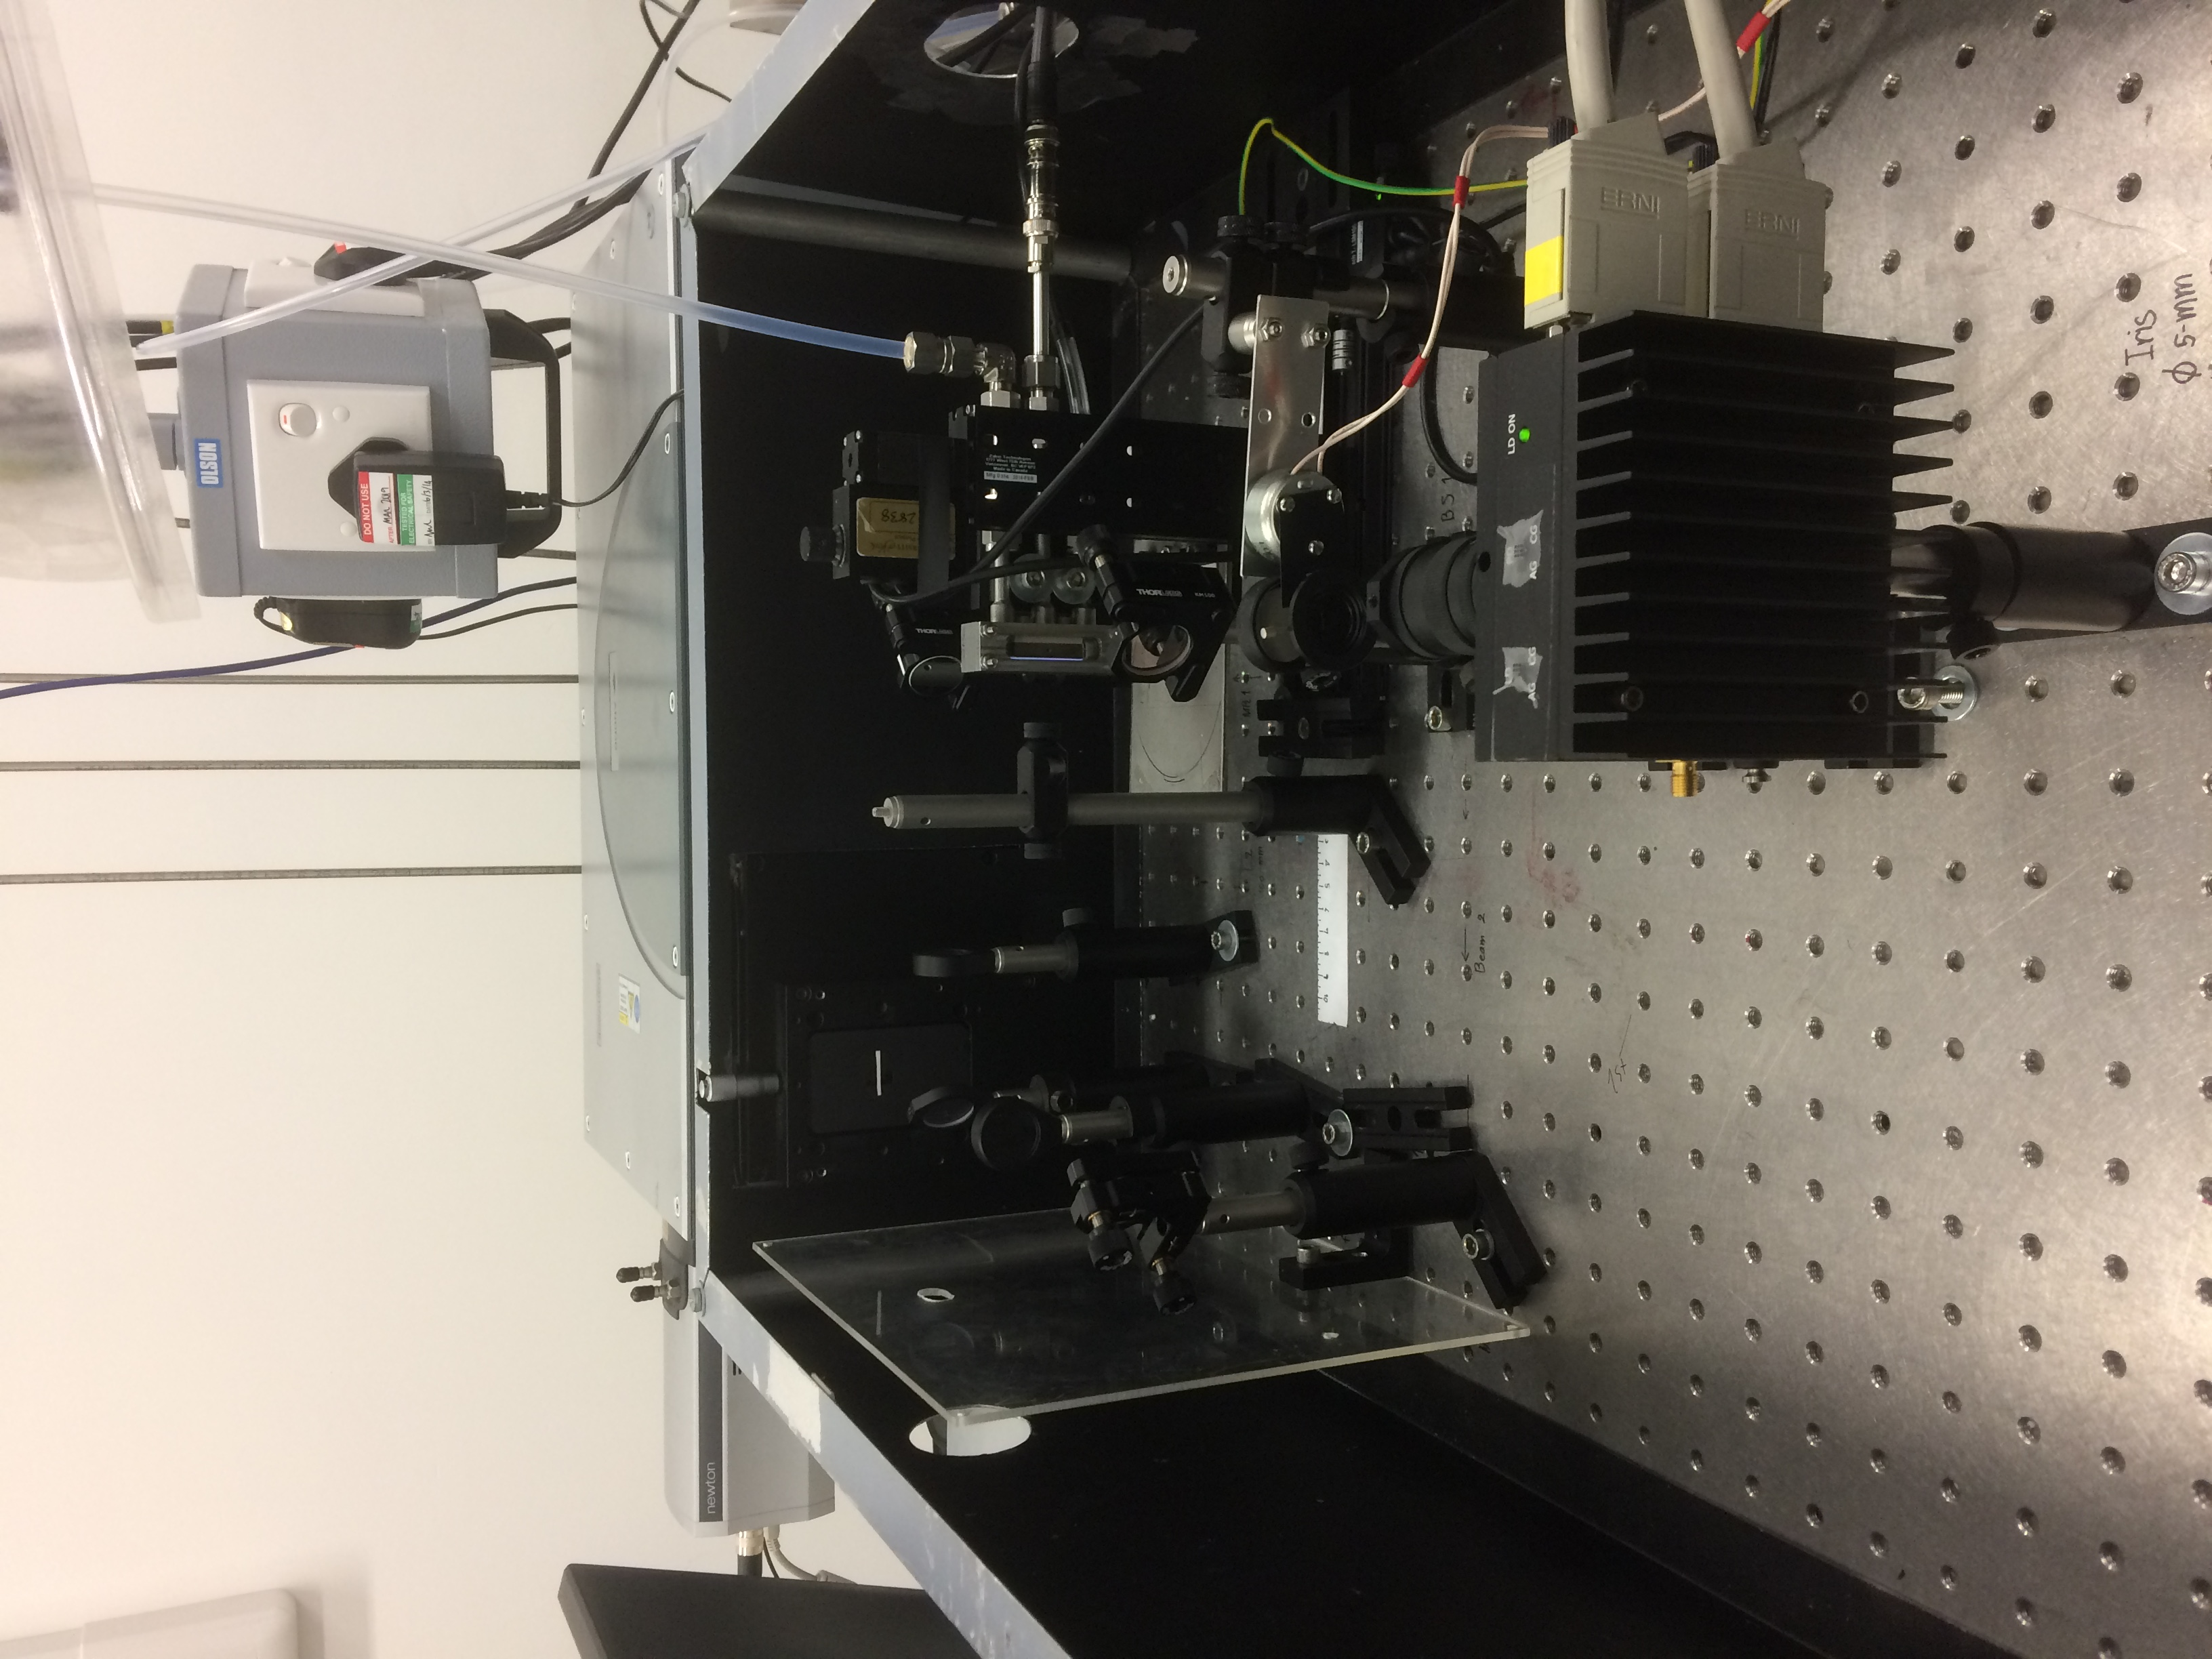
\includegraphics[width=\textwidth]{Figures/PlasmaSetup.JPG}
    \caption{Plasma Setup...This will be a proper diagram...}
    \label{fig:my_label}
\end{figure}


\subsection{Power Measurements}

Whilst the RF generator gives an indication of the power being supplied to the plasma source, it is not very accurate and is unable to account for power losses in cables and other equipment.
To counteract this, the actual power delivered to the plasma can be accurately measured using a Solayl probe which is connected between the matching box and the plasma source.
Using this, the actual power delivered to the plasma was calibrated to the output stated on the output dial (see figure \ref{fig:OutputDial}) of the RF generator. 
This was done by changing the output from 50 - 160 in steps of 10 on the RF generator output dial and measuring the power at each point 5 times, then taking the average power for each output.
For this, the plasma was operated with a gas flow of 5 slm helium containing 5400ppm water.
This calibration is shown in figure \ref{fig:SolaylPower}.
The relationship between the output and actual power showed a linear relationship and by fitting a line to the measured data, the actual power delivered to the plasma for each output value can be predicted. 
All powers stated in this report are real powers calculated from this calibration.

\begin{figure}
    \centering
    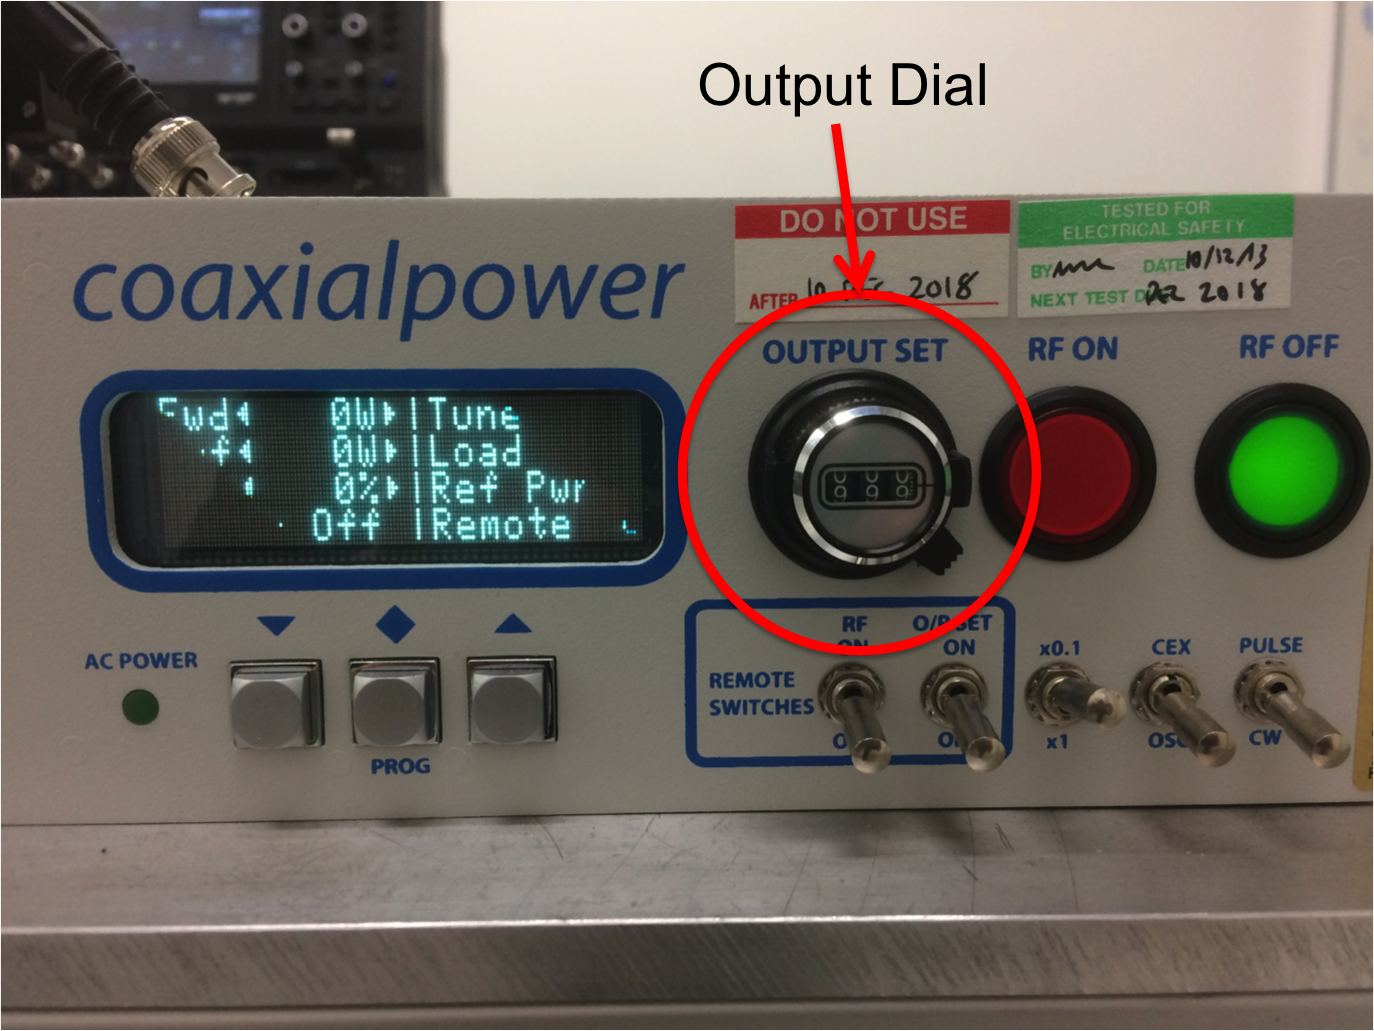
\includegraphics[width=0.4\textwidth]{Figures/OutputDial.png}
    \caption{Picture showing the Output dial on the RF generator used for calibrating output from the RF generator to the actual power supplying the plasma}
    \label{fig:OutputDial}
\end{figure}

\begin{figure}
    \centering
    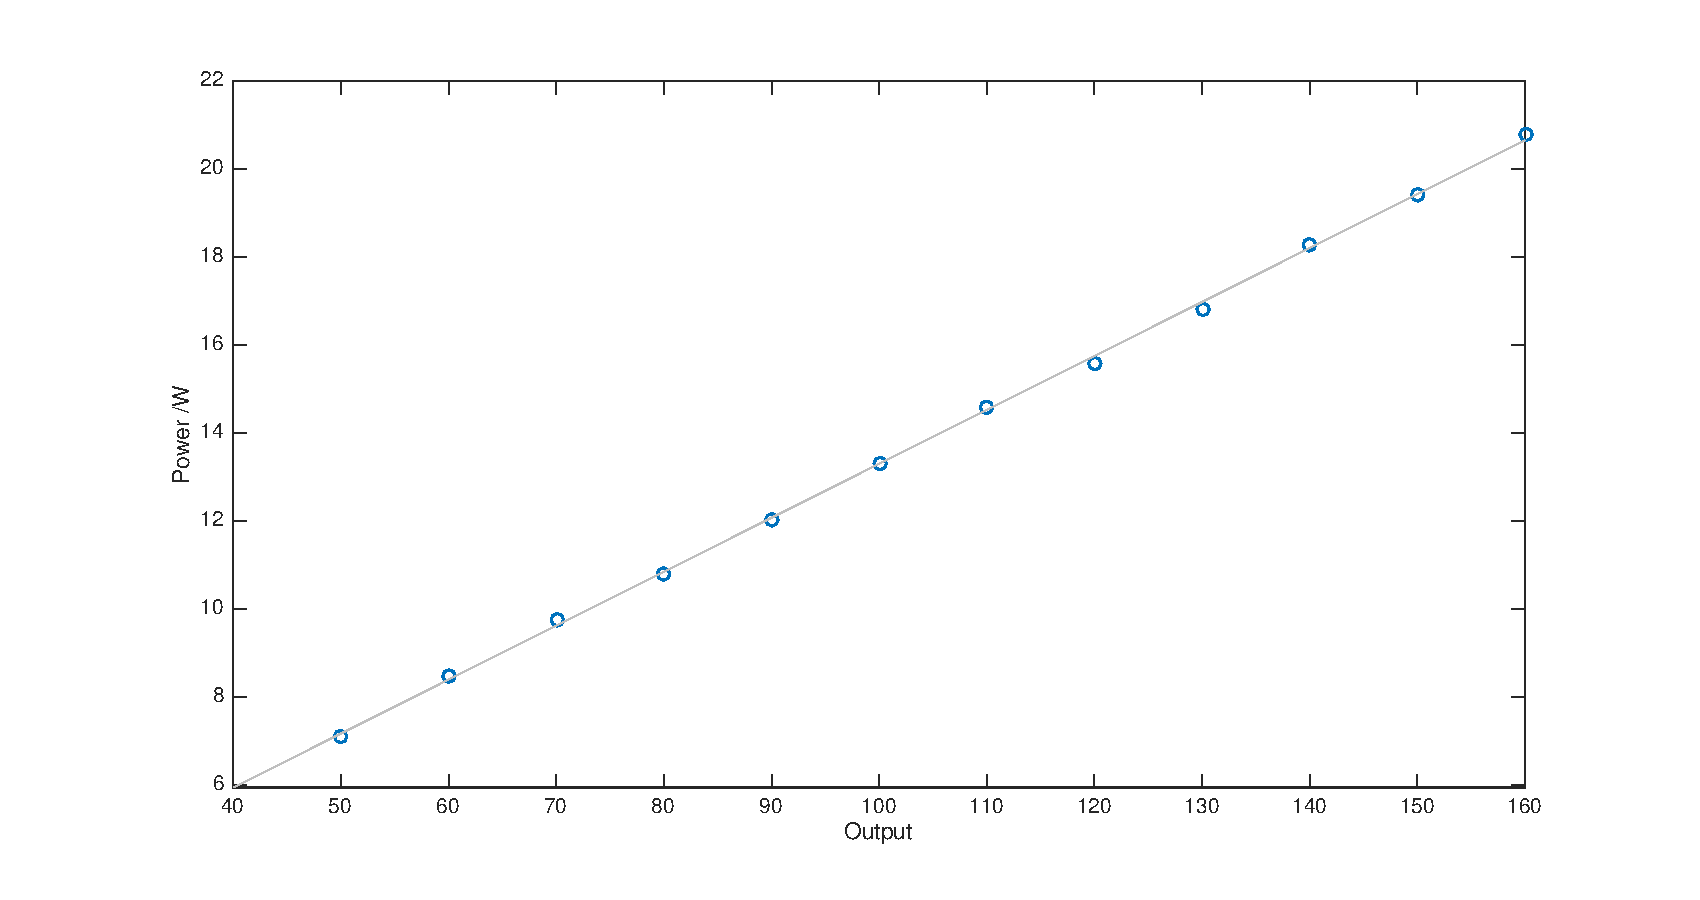
\includegraphics[width=\textwidth]{Figures/SolaylPower.eps}
    \caption{There is a linear relationship between the output on the RF generator and the actual power supplied to the plasma. The range of outputs for the plasma set up is 58-97. Using the equation of the line of best fit (y = 0.1227x + 1.0229) this equates to a power range of 8.1-12.9W. Powers shown are the average of 5 measurements.}
    \label{fig:SolaylPower}
\end{figure}

Following this calibration, it was necessary to check that the power delivered to the plasma was unaffected by changing the water content of the feed gas by altering the proportion of the 5 slm helium which is passed through the bubbler.
This was checked at two different powers. 
For each power, the RF generator output was kept constant and the volume of helium passing through the bubbler was varied.
The results shown in figure \ref{fig:BubblerPower} show that the water content has very little, if any effect on the power supplied to the plasma.

\begin{figure}
    \centering
    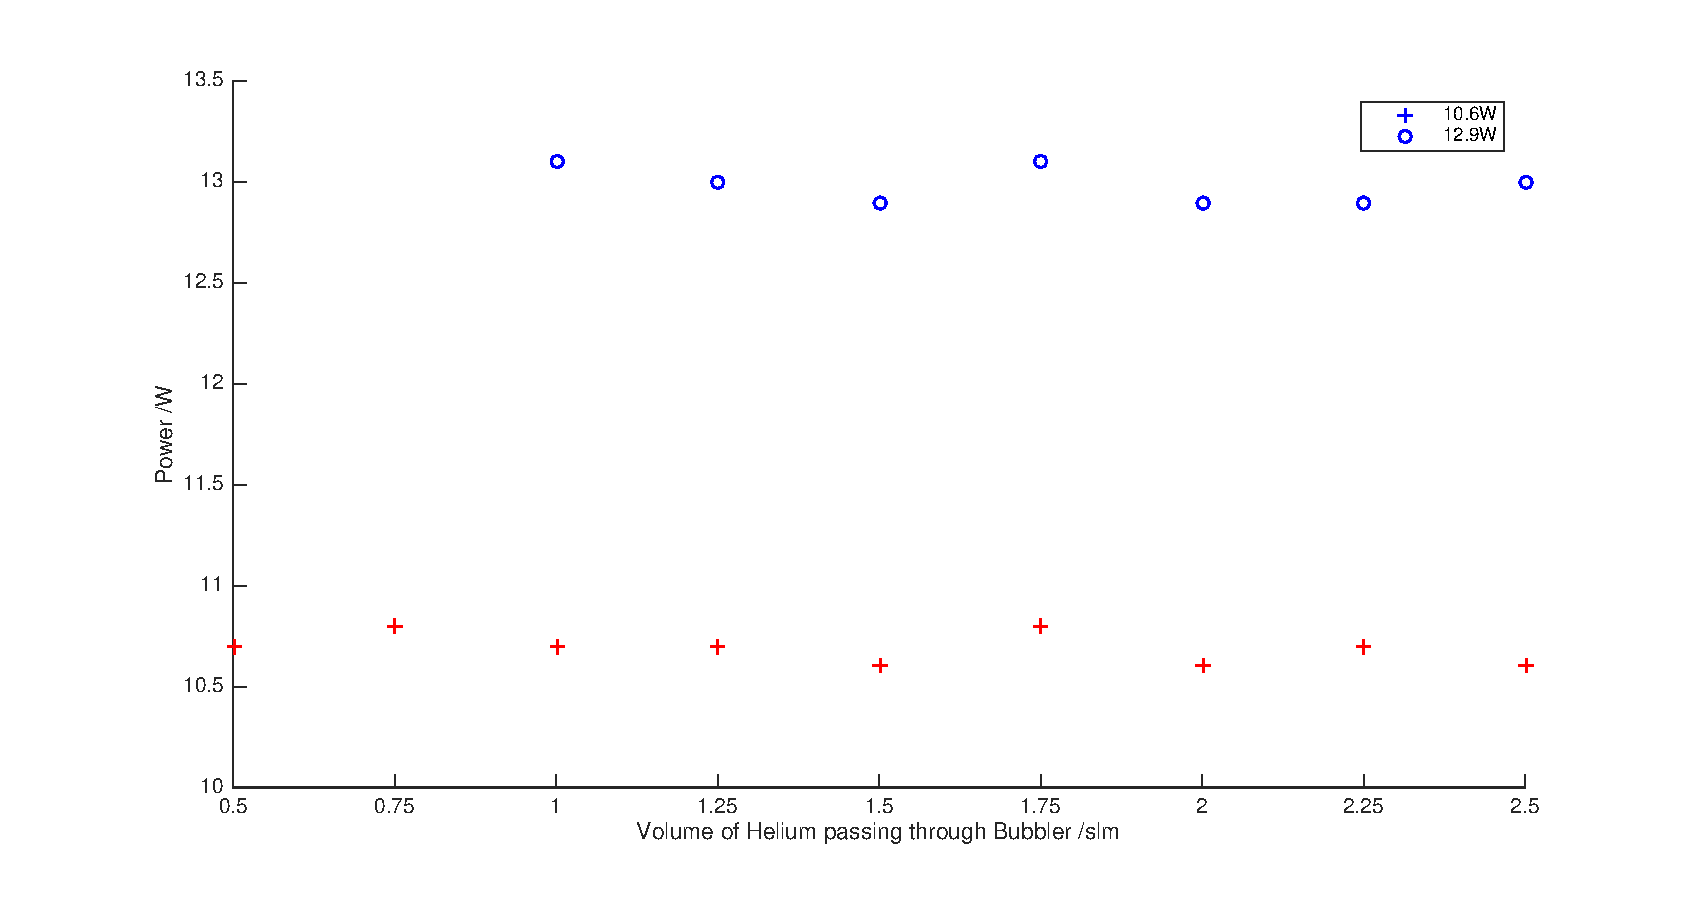
\includegraphics[width=\textwidth]{Figures/BubblerPower.eps}
    \caption{The water content of the feed gas has no effect on the power supplied to the plasma. The water content of the feed gas was varied at high and low power. For each of the two powers, the output of the RF generator was kept constant and only the water content of the feed gas changed.}
    \label{fig:BubblerPower}
\end{figure}

\subsection{UV Absorption Spectroscopy}
To investigate the density of hydroxyl radicals present in the plasma, an ultraviolet (UV) light emitting diode (LED) with central wavelength of 309 nm (a wavelength absorbed by free hydroxyl radicals (Hatano2010)) was used for absorption spectroscopy.
The principle of this method is to measure the intensity of light before and after passing through the plasma, in order to see how much has been absorbed within the plasma by the species of interest.
In this case, the species of interest is the hydroxyl radical, therefore, the more hydroxyl radicals present in the plasma, the greater the absorbance of LED.
The UV beam passes through the plasma and a series of optics, then signal is detected by an imaging spectrograph with a (CCD) camera.

The transmittance of light beam and it's relationship to the absorbance is shown as follows:


\begin{equation} \label{eqn:Transmittance}
    T = \frac{I_T}{I_0} = e^{-A}
\end{equation}
Where $T$ is transmittance, $I_T$ and $I_0$ are the intensities of the transmitted and incident light, respectively and $A$ is the absorbance of light by the plasma.

In order to measure $I_T$ and $I_0$ for the plasma setup, it is necessary to measure four different parameters as follows:
\begin{itemize}
    \item $I_{PL}$ - The intensity of light reaching the CCD when both the LED and the plasma are on (figure \ref{subfig:Ipl})
    \item $I_{P}$ - The intensity of light reaching the CCD when the LED is off and the plasma is on (figure \ref{subfig:Ip})
    \item $I_L$ - The intensity of light reaching the CCD when the LED is on and the plasma is off (figure \ref{subfig:Il})
    \item $I_{BG}$ - The intensity of background light when both the LED and plasma are off (figure \ref{subfig:Ibg})
\end{itemize}

\begin{figure}
	\begin{subfigure}{0.2\textwidth}
  	  	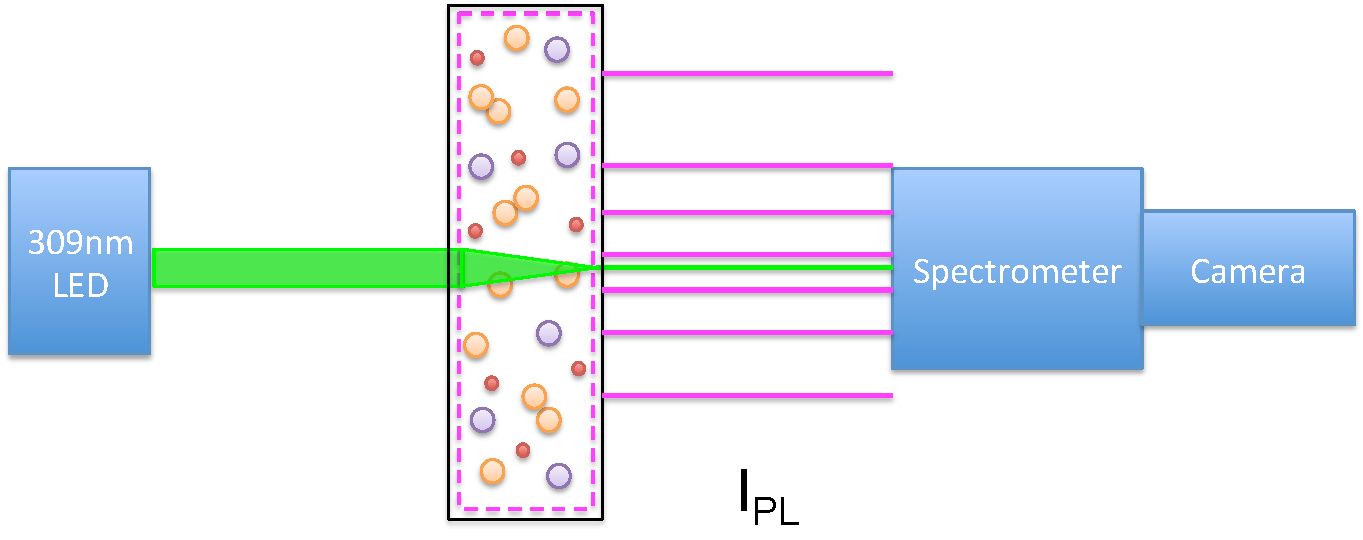
\includegraphics[width=\textwidth]{Figures/Ipl.pdf}
   	 	\caption{$I_{PL}$}
    		\label{subfig:Ipl}
	\end{subfigure}
	\hfill
	\begin{subfigure}{0.2\textwidth}
    		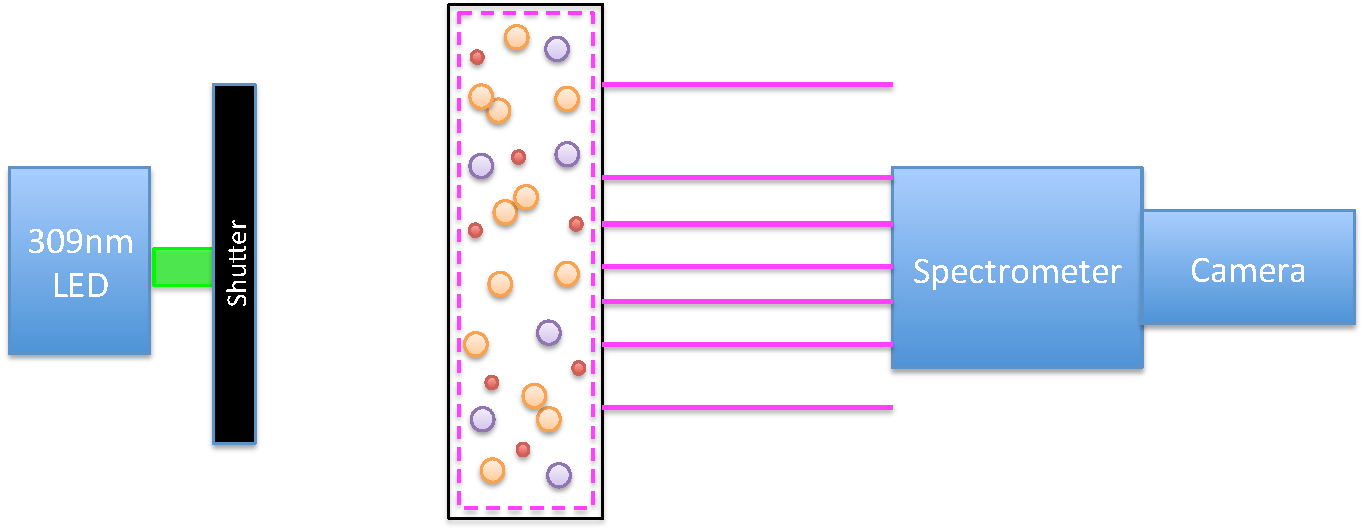
\includegraphics[width=\textwidth]{Figures/Ip.pdf}
    		\caption{$I_{P}$}
    		\label{subfig:Ip}
	\end{subfigure}
	\hfill
	\begin{subfigure}{0.2\textwidth}
		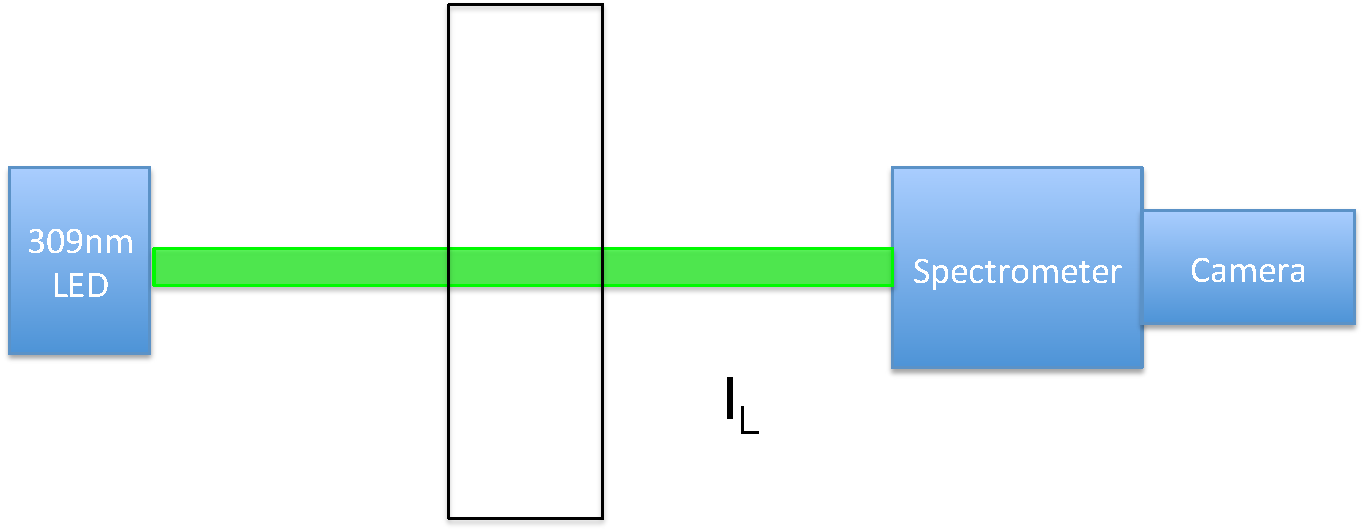
\includegraphics[width=\textwidth]{Figures/Il.pdf}
    		\caption{$I_{L}$}
		\label{subfig:Il}
	\end{subfigure}
	\hfill
    	\begin{subfigure}{0.2\textwidth}
    		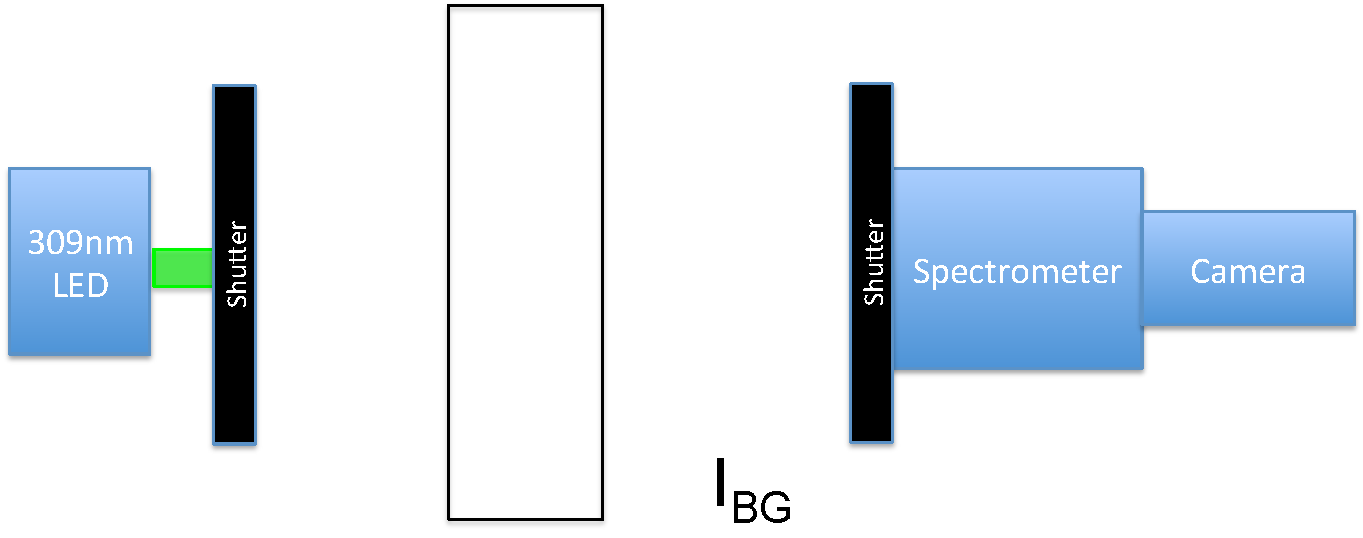
\includegraphics[width=\textwidth]{Figures/Ibg.pdf}
    		\caption{$I_{BG}$}
    		\label{subfig:Ibg}
	\end{subfigure}
	\caption{Rectangle represents plasma channel. Splodges are important bits of plasma. Green line is LED.}
\end{figure}

Using these measurements, the equation defining the relationship between transmittance and absorbance becomes:

\begin{equation} \label{eqn:4ParamTransmittance}
    T = \frac{I_T}{I_0} = \frac{I_{PL} - I_P}{I_L - I_{BG}} = e^{-A}
\end{equation}

All four parameters are measured in series, under the control of a function generator.
This function generator controls a shutter to block the LED and the RF generator to turn the plasma on and off. It also controls external triggering of the camera and a shutter at the entrance to the spectrometer to block all light to the CCD while the system changes from one parameter to the next. 

Data is then acquired as a series of 80 measurements resulting in 20 repeats for each of the four parameters.
Matlab is then used to average all 20 repeats for each parameter then calculate absorbance at each wavelength of the LED as follows:

\begin{equation}\label{eqn:Absorbance}
    A = -ln(\frac{I_{PL} - I_P}{I_L - I_{BG}})
\end{equation}

\subsection{Spectral fitting and radical density determination}

Once the absorbances for each wavelength have been calculated, a simulated spectrum can then be fitted to the data to provide a spectrum of absorbance for hydroxyl radicals (see figure \ref{fig:SpectrumFitting}). 
The spectrum shows absorption due to ground state hydroxyl radicals becoming rotationally and/or vibrationally excited.
In fitting this spectrum, the programme calculates the density of hydroxyl radicals present in the plasma.

\begin{figure}
    \centering
    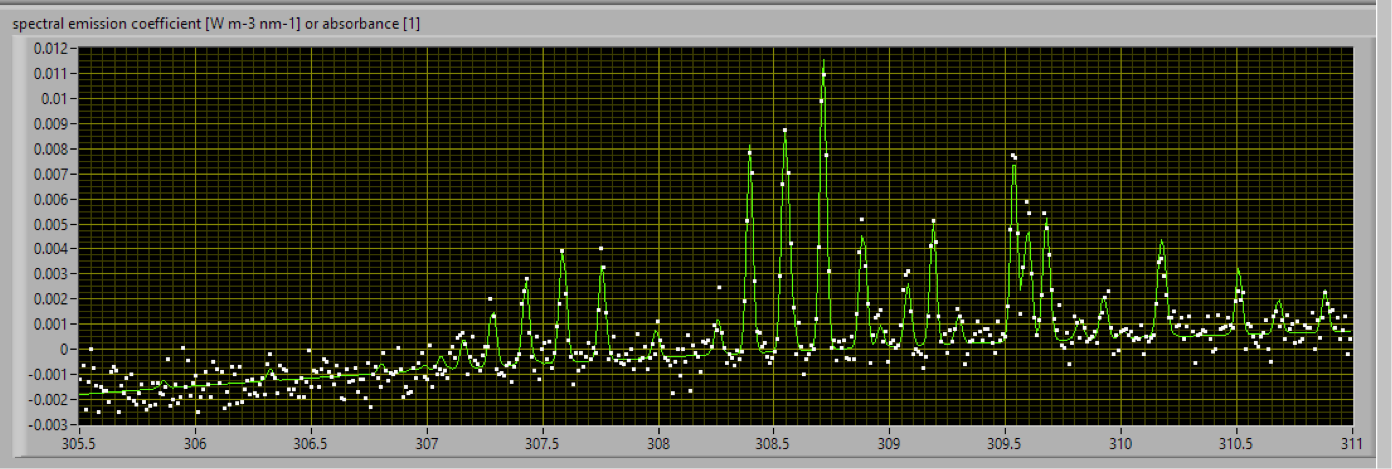
\includegraphics[width=\textwidth]{Figures/SpectrumFitting.png}
    \caption{An example of a simulated spectrum (green) fitted to the measured absorbances (white dots). Wavelength is shown along the x axis and absorbance along the y axis.}
    \label{fig:SpectrumFitting}
\end{figure}

\subsection{Calculating the Water Content of Helium}
\label{subsec:CalculatingWaterContent}


To calculate the water content of helium passing through the bubbler, firstly, the flow of water must be determined. For this, the pressure of water vapour in the bubbler ($P_{water}$) is calculated using the following:

\begin{equation}
	e_w = 6.1094 e^{\frac{17.625t}{243.04 + t}}
\end{equation}
Where $e_w$ is the water vapour pressure in hPa, above a plane surface of pure water, and $t$ is the temperature in degrees celsius.

The pressure of helium ($P_{He}$) is taken to be $P_{atmosphere} - P_{water}$. Since the ratio of flow to pressure for helium must be the same as for water, the flow of water can be calculated as follows:

\begin{equation}
    F_{water} = \frac{F_{He} * P_{water}}{P_{He}}
\end{equation}

Where $F_{water}$ and $F_{He}$ are the flows of water and helium in slm, respectively. The percentage of gas flow that is water, and the concentration of water in parts per million can then be determined.
The relationship between the flow of helium through the bubbler and the concentration of water in ppm is shown in figure \ref{fig:WaterContent}.

\begin{figure}
    \centering
    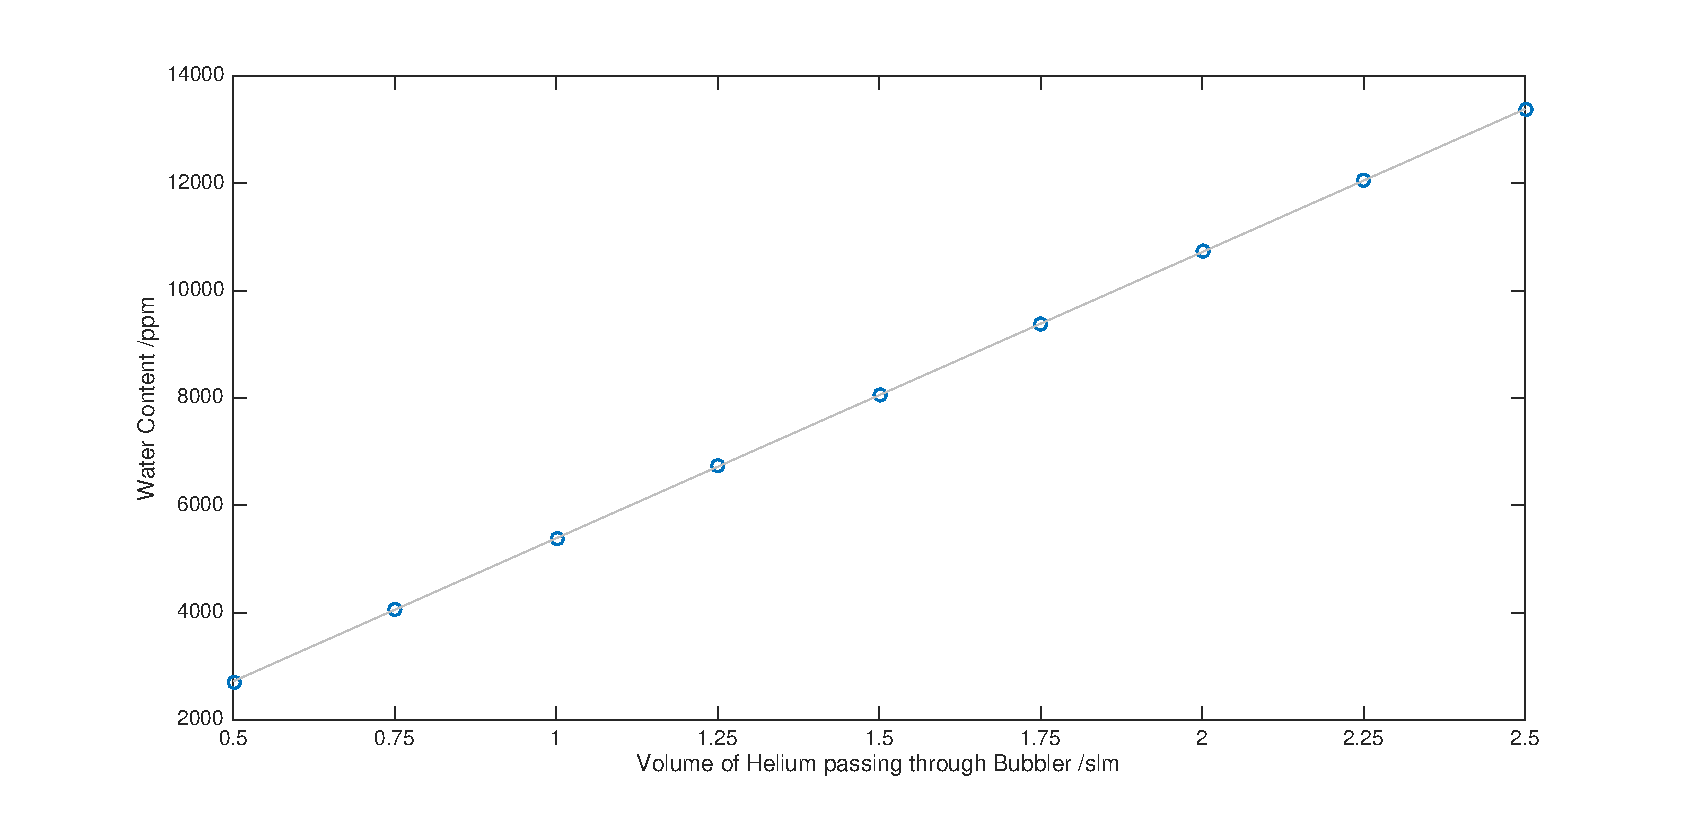
\includegraphics[width=\textwidth]{Figures/WaterContent.eps}
    \caption{The water content of the helium passing through the bubbler increases linearly with the volume of helium passing through the bubbler. Water content calculated using equation from Alduchov paper and procedure described in the text.}
    \label{fig:WaterContent}
\end{figure}

\subsection{Modelling of Hydroxyl Radical Production}

\begin{itemize}
\item Global model of plasma
\item approximately 300 reactions taken into account and the probabilities that they will occur
\item Coupled with gas flow rate, power, plasma volume and diffusion length
\item Solves equations that take into account radical losses at the edges and reactions which result in their formation again at the edges along with probabilities that they're produced in the first place (rate constant)
\item Running the model then can give an indication of the dominant reactions for the production and loss of hydroxyl radicals
\end{itemize}



\section{Results}

\subsection{Spatial Resolution of Hydroxyl Radicals}

\begin{figure}
    \centering
    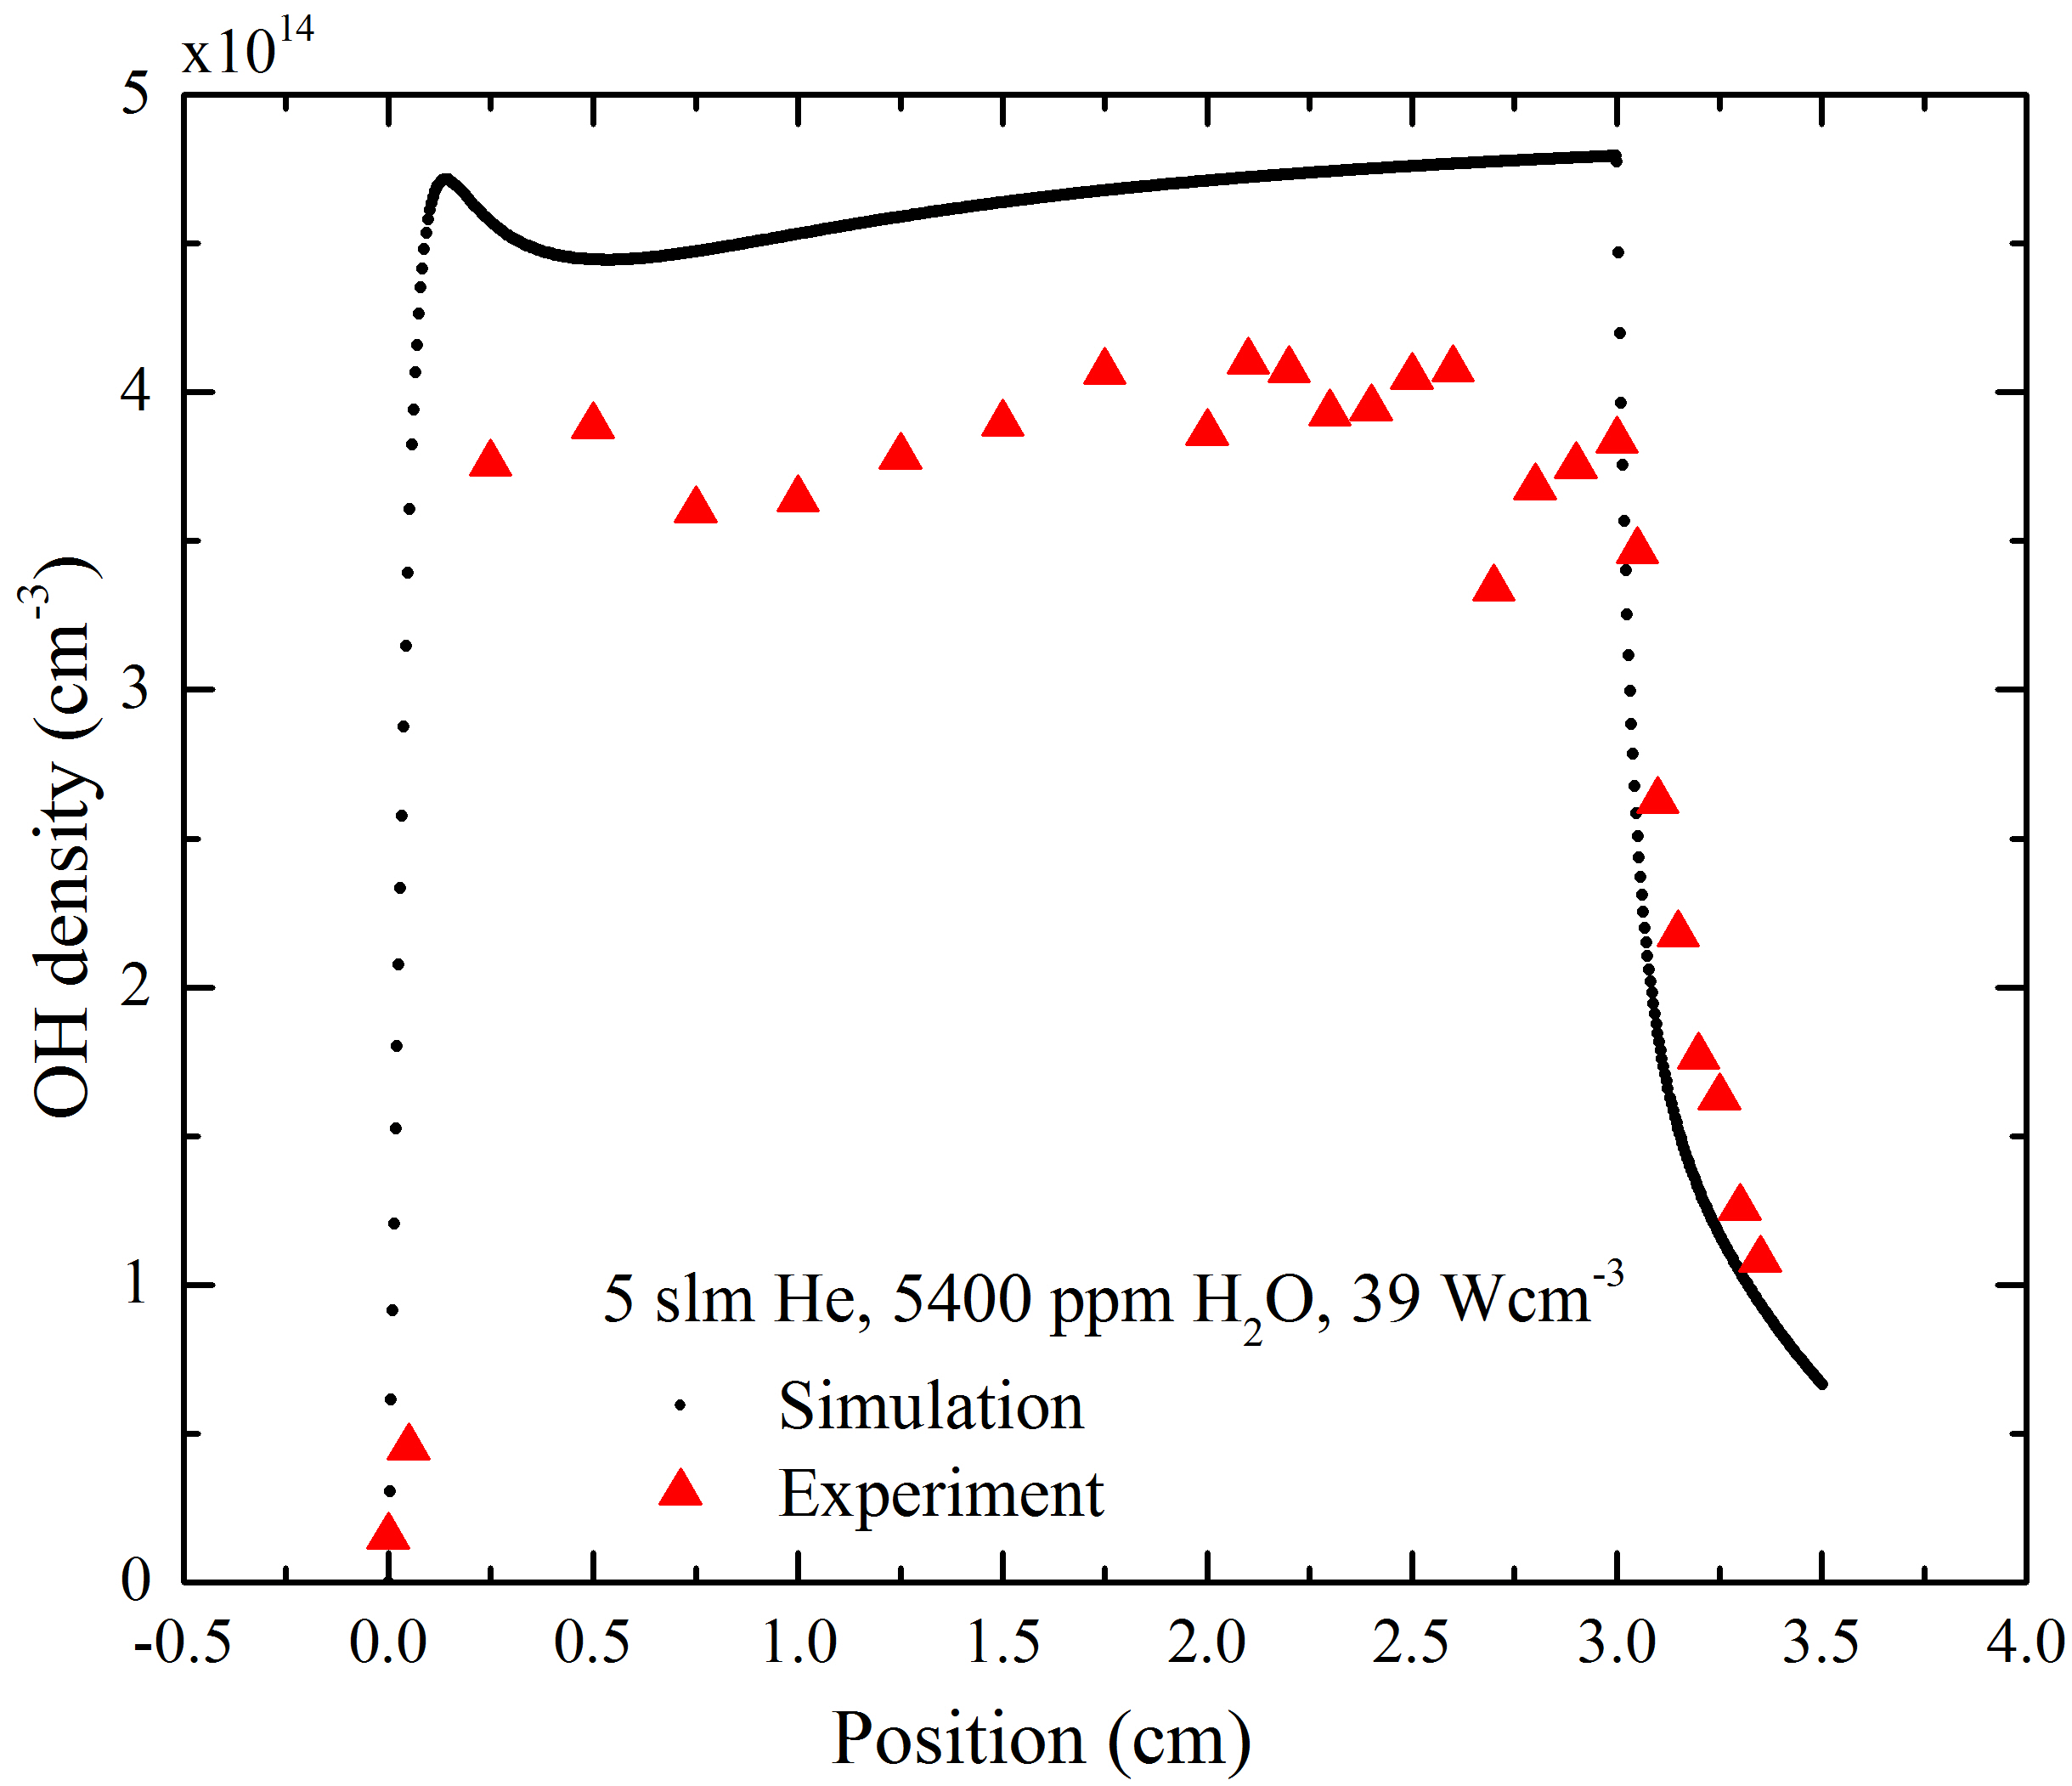
\includegraphics[width=\textwidth]{Figures/OHSpatialwithSim.jpg}
    \caption{Figure showing the effects of distance from gas inlet on the density of hydroxyl radicals in plasma. Absorption spectroscopy was performed at 0.5-1mm intervals along the 30mm length of the electrodes (0-30mm), plus at 0.5mm intervals beyond the end of the plasma region (30.5-33.5mm). This was performed at the maximum power for the plasma before arcing occurs. A total gas flow of 5 slm helium was used with 5400ppm water.}
    \label{fig:SpatialRes}
\end{figure}

\begin{figure}
	\centering
	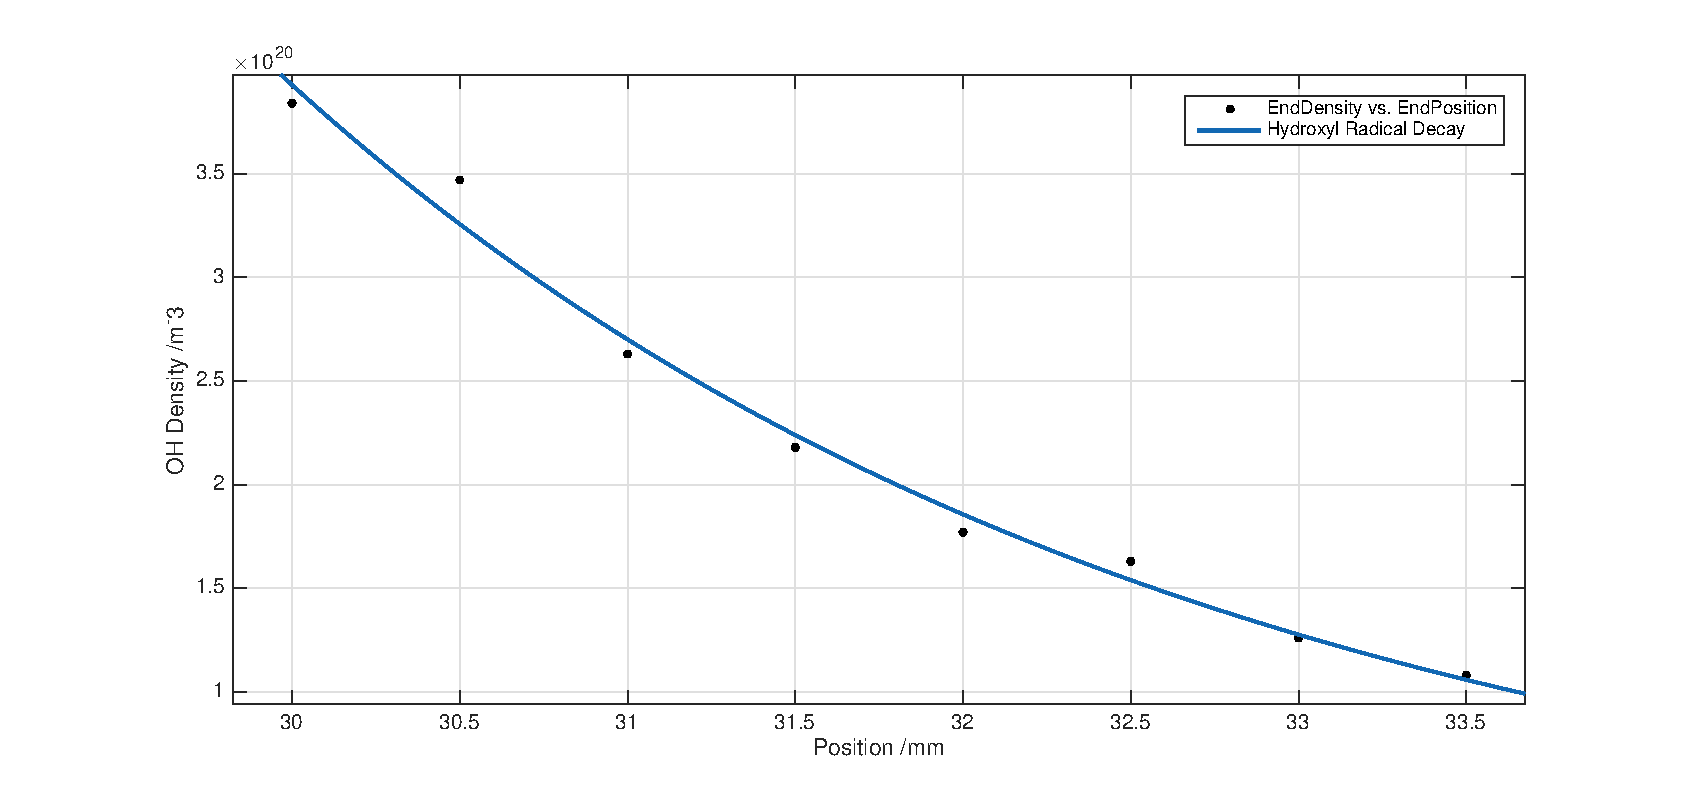
\includegraphics[width=\textwidth]{Figures/OHdecay.eps}
	\caption{Figure showing how the density of hydroxyl radicals falls away exponentially beyond the electrodes. The 30mm point is the end of the electrodes and 33.5mm is the last point where the measurement could be taken before the LED was blocked by the casing of the plasma source.}
	\label{fig:OH decay}
\end{figure}


The aim of this is to show how the distance from the gas inlet, and therefore, position along the 30mm electrode, affects the density of hydroxyl radicals. Figure \ref{fig:SpatialRes}.
It also is able to provide information on the decay rate of hydroxyl radicals at the end of the electrodes.
Also able to compare to simulated data.
Data acquired using a power of Op97 which is the maximum power that can be applied to the plasma before arcing occurs.
\begin{itemize}
    \item Sharp increase from 0-2.5mm, followed by a smaller increase and decrease to give a little hump seen in both the experimental and simulated data. Following this there is an increase in density over the rest of the channel. The change is very small (less than 1 x 1020 m-3)
   
    \item Significant decrease in hydroxyl radical density beyond the end of the electrodes. Distance is not sufficient to allow the density to decrease to the densities seen at the very start of the electrodes. 
        
    \item To interrogate the decrease beyond the end of the electrodes, the measurements were taken every 0.5mm from the end of the channel to the edge of the casing. A curve was then fitted to the data points to see the decay of hydroxyl radicals with distance from the end of the electrodes
    
    \item Have to be careful to say this is the true decay though as the whole casing of the plasma source acts as the grounded electrode so in fact, the ends of the electrodes will still be interacting with the grounded casing around the ends of the electrode.
    
    \item However, very nice exponential decay curve can be drawn for the decay. Half distance (like half life but in distance rather than time!!!) is approximately 1.9mm!
    
    \item By plotting the decay on a log scale, it gives an idea as to how many decay processes are occurring. For example, a linear relationship over the full decay would suggest that there is one dominant decay process. 
    In looking at the information provided by the model, the dominant reaction causing loss of OH is $OH + H_2O_2 \rightarrow  HO_2 + H_2O$. However, it also suggests that there are other processes that are less important but still contributing, in particular $OH +HO_2 \rightarrow O_2 +H_2O$ and  $OH + OH \rightarrow H_2O_2$.
\end{itemize}

Overall, both the experimental and simulated data show a similar trend over the full length of the plasma channel with a sharp increase at the beginning, a small increase and decrease between approximately 2.5 - 7 mm, followed by an overall slight increase in density to the end of the electrodes.
Beyond the electrodes the density seems to decrease quickly with a lifetime of ???????.
This very short lifetime is due to the fact that hydroxyl radicals react very readily with everything and are therefore lost.


\subsubsection{The percentage dissociation is very small}

The degree of dissociation of water to hydroxyl radicals was then investigated... 
This showed that the percentage dissociation (hydroxyl/water *100) was very small.
However, while these numbers seemingly show that only a small amount of the water is dissociating, it may also be that the hydroxyl is recombining with other things and therefore being lost.

\begin{figure}
	\centering
	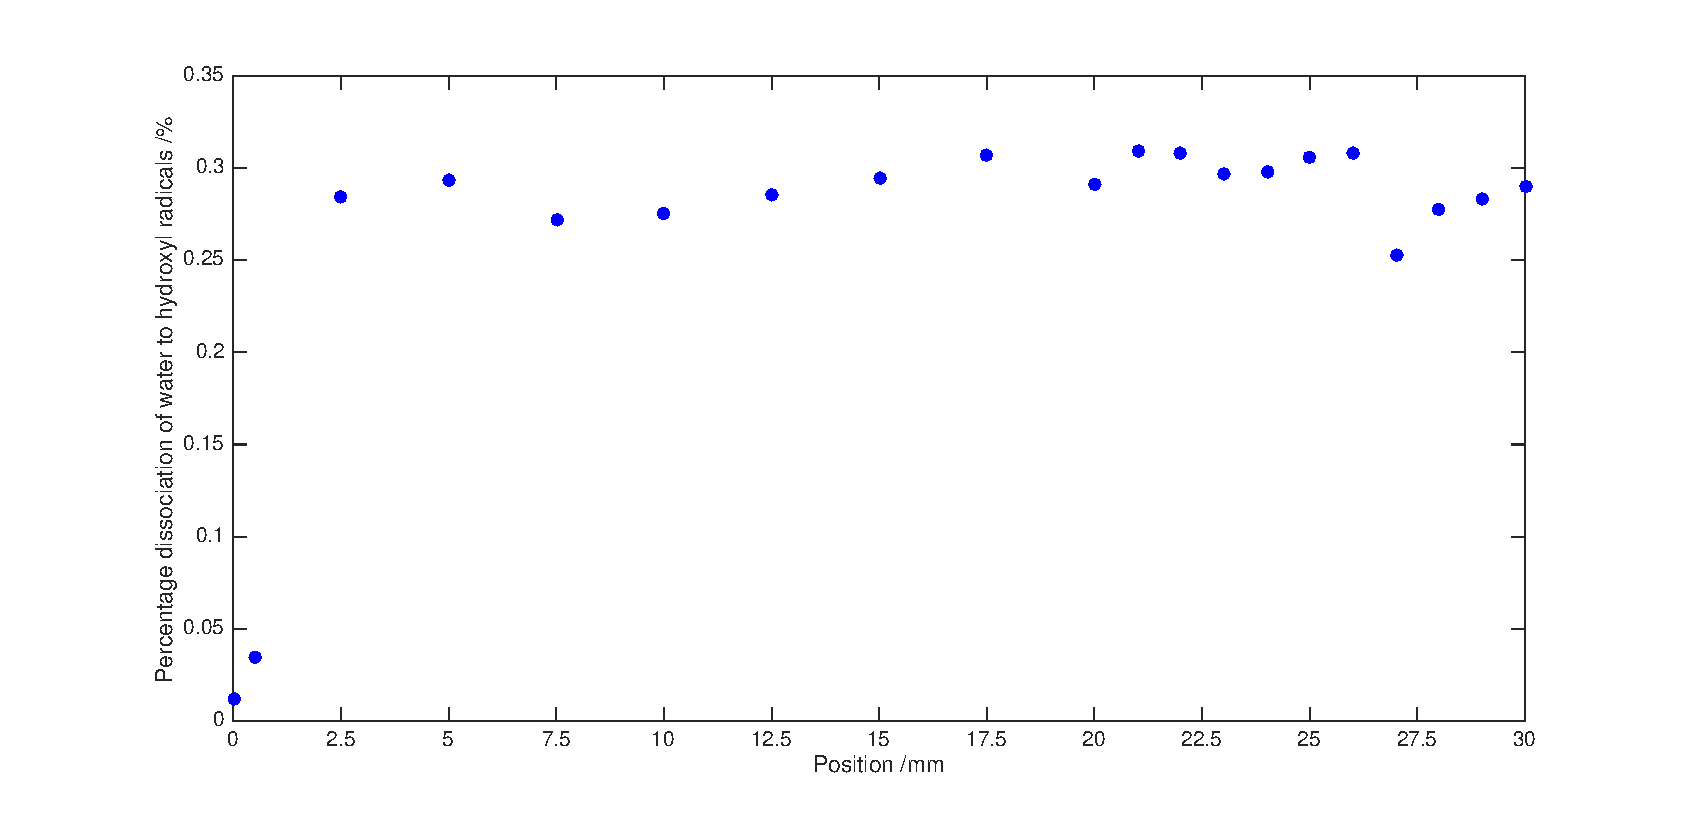
\includegraphics[width=\textwidth]{Figures/SpatialDissociation2.eps}
	\caption{The figure shows the percentage dissociation of water to hydroxyl radicals, calculated as ppm hydroxyl radicals divided by ppm water in, all multiplied by 100. Since the ppm of water stays the same at all positions, the graph shows the same trend as the equivalent density graph.}
	\label{fig:SpatialDissociation}
\end{figure}


\subsection{Increasing the power to the plasma increases hydroxyl radical density}

Following investigation of the spatial resolution of hydroxyl radicals, the effects of power variation were then investigated.
It was of interest to see how varying the power would affect the density of hydroxyl radicals and the percentage dissociation of water to hydroxyl.
The 20mm position was chosen to investigate as at this point, the densities of hydroxyl radical seems to level off slightly. 
The full range of powers for the plasma were tested from ????? (minimum power for sustaining the plasma) to ????? W (maximum power before arcing occurs).

The results of this are shown in figure \ref{fig:PowerVariation}.

\begin{figure}
    \centering
    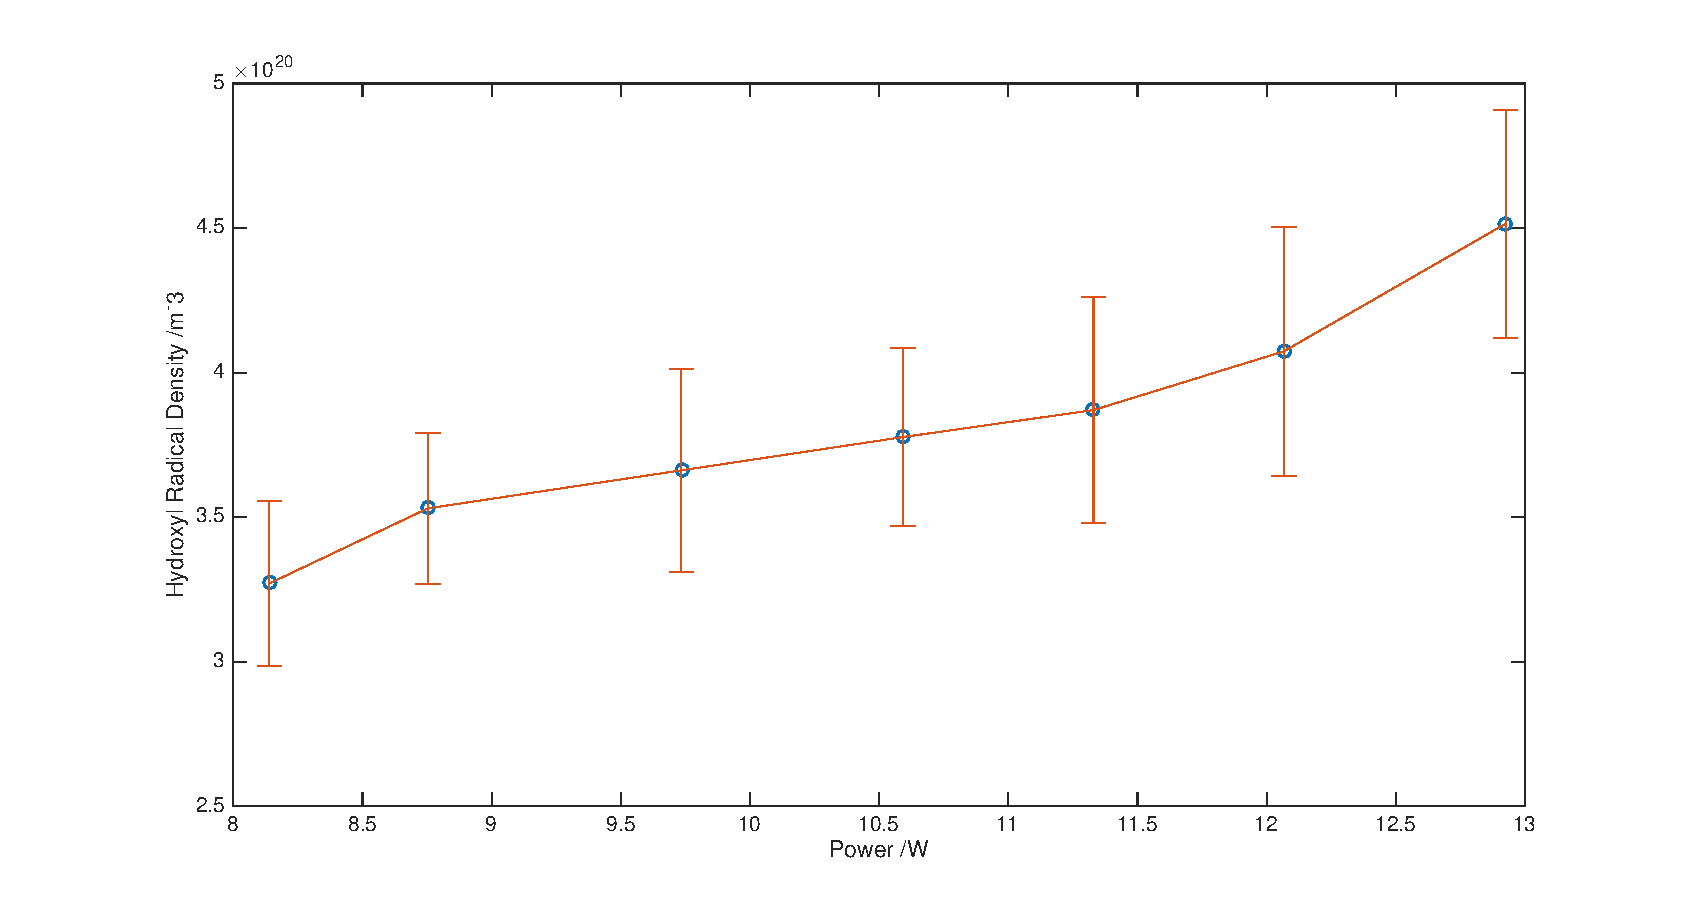
\includegraphics[width=\textwidth]{Figures/PowerVariation.eps}
    \caption{Power increases hydroxyl radical density in the plasma region in a non-linear manner. Absorption spectroscopy was performed at a point 20mm from the gas inlet while power being dissipated in the plasma was varied within the range of ????8.1-12.9W???. Total gas flow to the plasma was kept constant at 5slm helium with 5400ppm water. The experiment was repeated four times. The graph shows the average density for each power and the error bars represent one standard deviation.}
    \label{fig:PowerVariation}
\end{figure}

\begin{itemize}
    \item Densities increase non-linearly from min to maximum power.  Density at min and max power are similar to those seen in spatial resolution data, at least, within the error.
    \item Density range of approximately 3.25 - 4.5 x 10\textsuperscript{20} m\textsuperscript{-3}
    \item Experiment repeated 4 times ? gives indication of expected error of approximately +/- 0.5 x 10\textsuperscript{20} m\textsuperscript{-3}.
\end{itemize}

\subsubsection{Dissociation}

The dissociation of water to hydroxyl radicals was then investigated for this experiment and, once again, the percentage dissociations were extremely small, though they did increase for the increased power. 
Unfortunately, the power cannot be increased any more for this setup before arcing occurs therefore increasing the dissociation would have to be achieved a different way. ?Increasing frequency may be a possibility.

\begin{itemize}
    \item Percentage dissociation increases with increasing power.
    \item Unfortunately, 12.9W is the maximum power achievable before arcing occurs in the plasma. It may be that without increasing the power it is not possible to increase the percentage dissociation. ?Increase frequency.
    \item Percentage is extremely small. This may be due to the very short lifetime of hydroxyl radicals which ultimately become more stable species. While it appears that the dissociation of water to .OH is very small, it may be that the water dissociates to .OH then the .OH is very quickly lost to other species making it undetectable. Would it be possible to measure water in the plasma to see how much is lost/left undissociated?
\end{itemize}

\begin{figure}
    \centering
    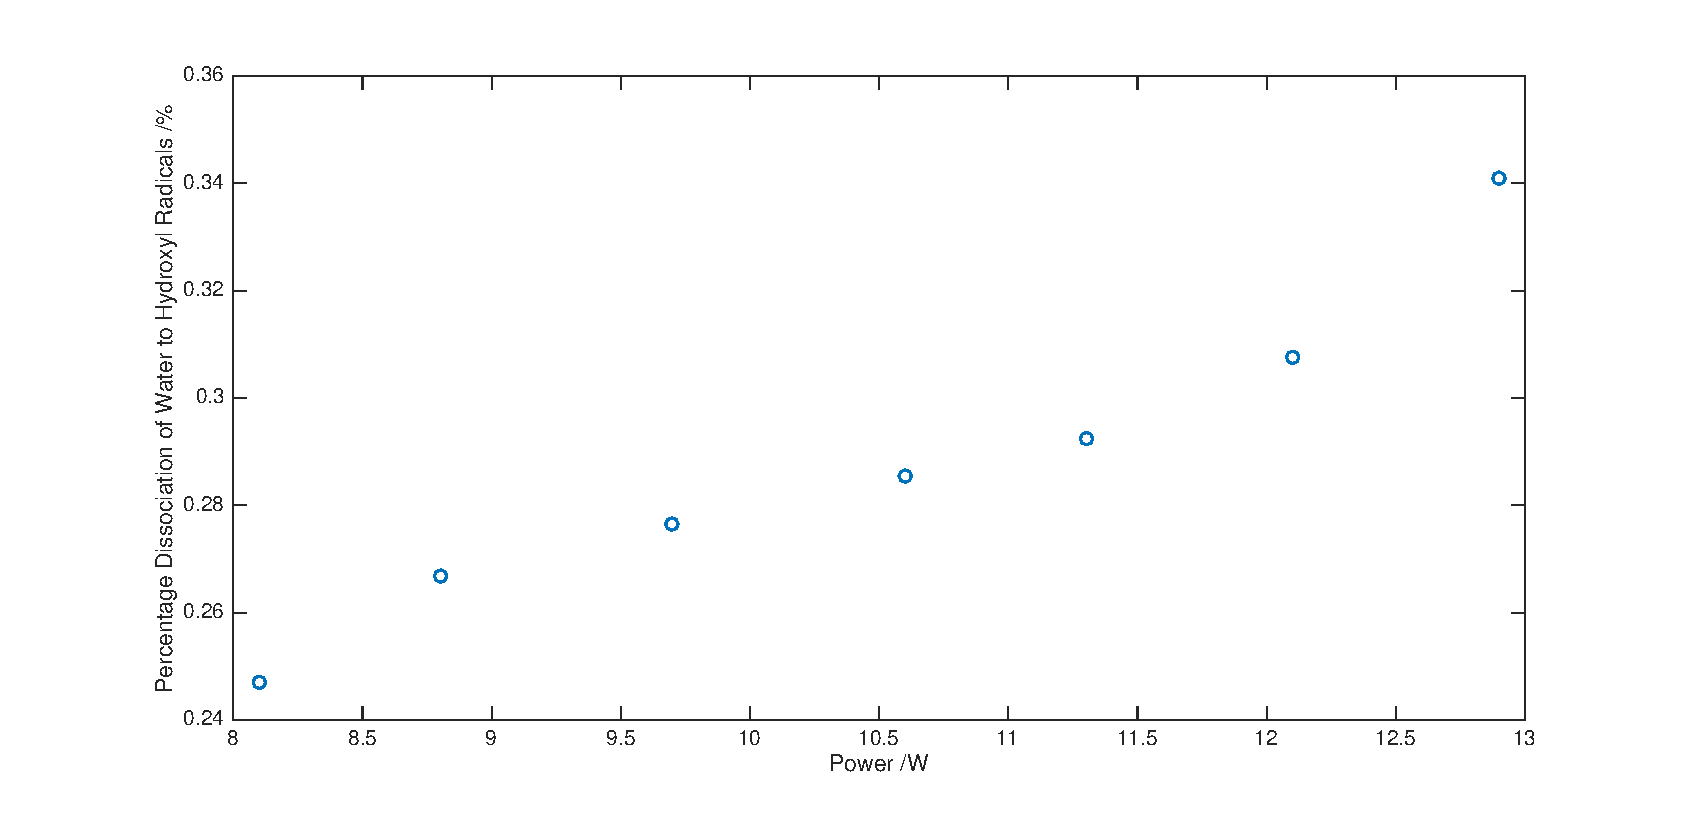
\includegraphics[width=\textwidth]{Figures/PowerDissociation.eps}
    \caption{Percentage dissociation of water to hydroxyl radicals increases with increasing power. Absorption spectroscopy was performed at a point 20mm from the gas inlet. The plasma was operated with a total gas flow of 5slm helium plus 5400ppm water. The percentage dissociation was calculated using the average density of hydroxyl radicals as shown in figure \ref{fig:PowerVariation}. The power range was ??8.1-12.9W??.}
    \label{fig:PowerDissociation}
\end{figure}

\subsection{Increasing the water content of the plasma gas feed increases hydroxyl radical density}

To investigate whether increasing the water being fed to the plasma increases the hydroxyl radical density, the ratio of dry and humid helium entering the plasma channel was altered by changing the proportion of the total 5 slm helium that passed through the bubbler. The range of water concentrations entering the plasma was approximately 2700 - 13400 ppm. The results are shown in figure \ref{fig:BubblerVariation}.

The powers had to be carefully chosen due to the effects of adding in additional molecules into the plasma which can act as energy sinks when they absorb energy to change rotational and vibrational states. 
Therefore, higher water contents require higher powers to ignite as the system becomes less efficient when more molecules are added.
Two different powers were used to investigate the effects of altering the water content. Firstly, ??W was used as this was sufficient to sustain the plasma at high water contents, without causing arcing at low contents. Secondly, the power was increased to see how the density increased at the higher power. 

\begin{figure}
    \centering
    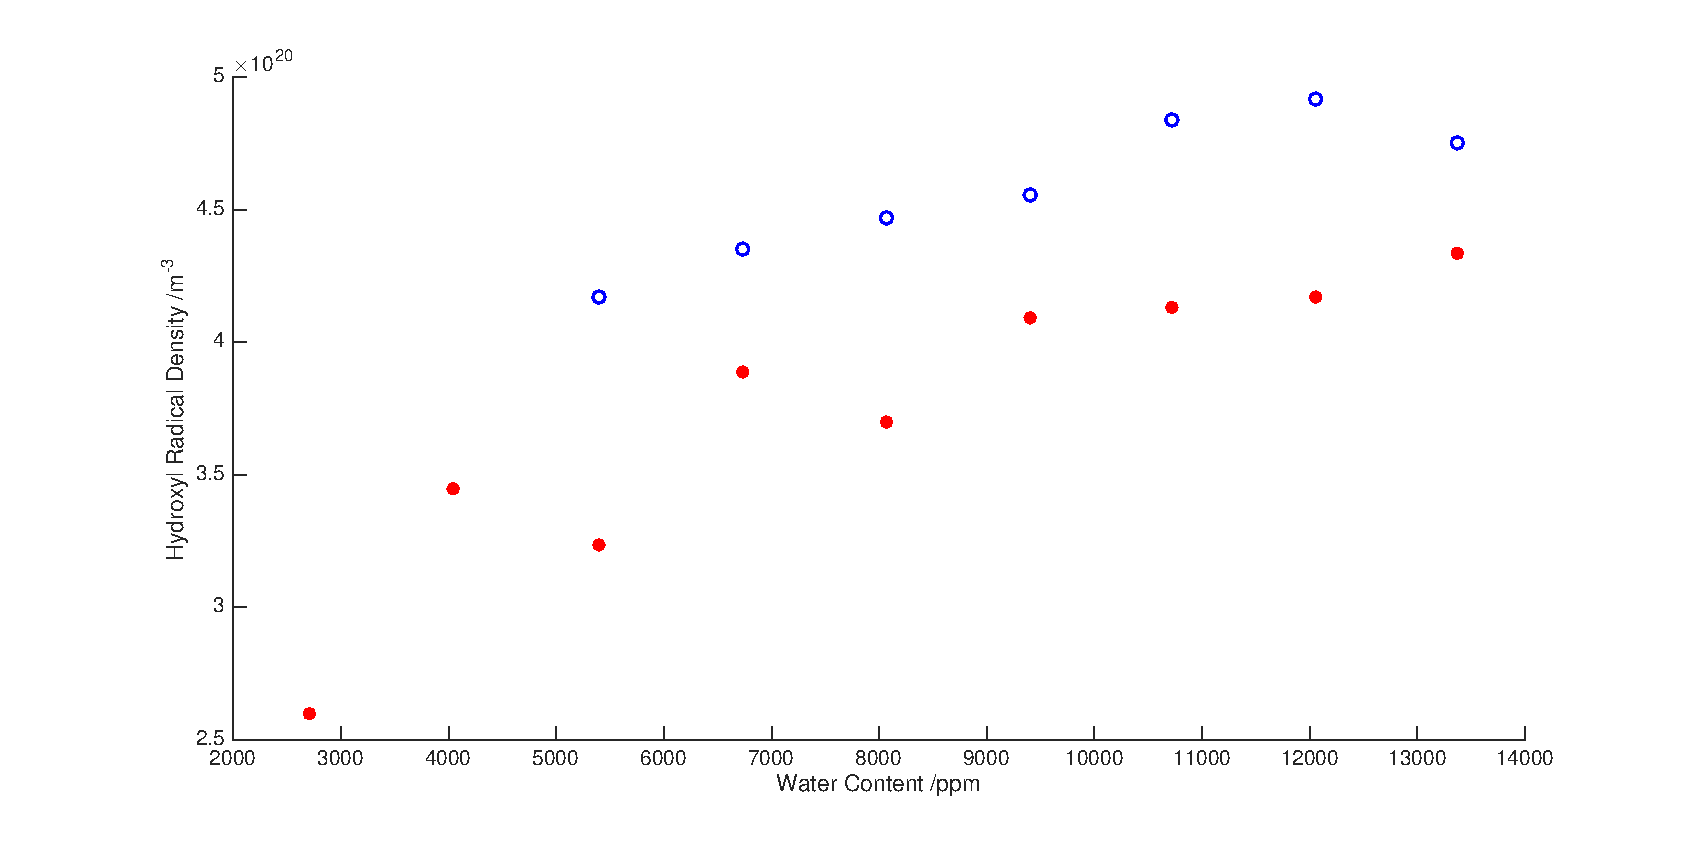
\includegraphics[width=\textwidth]{Figures/BubblerVariation}
    \caption{Increasing the water content of the helium entering the plasma channel increases hydroxyl radical density. Absorption spectroscopy of plasma at 20mm from the gas inlet was performed with different ratios of ?dry? and ?humid? helium entering the plasma channel. A total gas flow of 5 slm was maintained throughout. The range of water contents of the gas feed was approximately 2700 - 13400 ppm. The powers used were ??10.6W?? and ??12.9W??}
    \label{fig:BubblerVariation}
\end{figure}

\begin{itemize}
    \item Increasing the water content in the feed gas to the plasma increases the hydroxyl radical density
    \item The same trend is seen at both the lower and higher powers, though the densities are consistently higher at the higher power as expected. 
\end{itemize}

\subsubsection{Dissociation}

Look at how percentage dissociation changes with amount of water in plasmas. Figure \ref{fig:BubblerDissociation}.

\begin{figure}
    \centering
    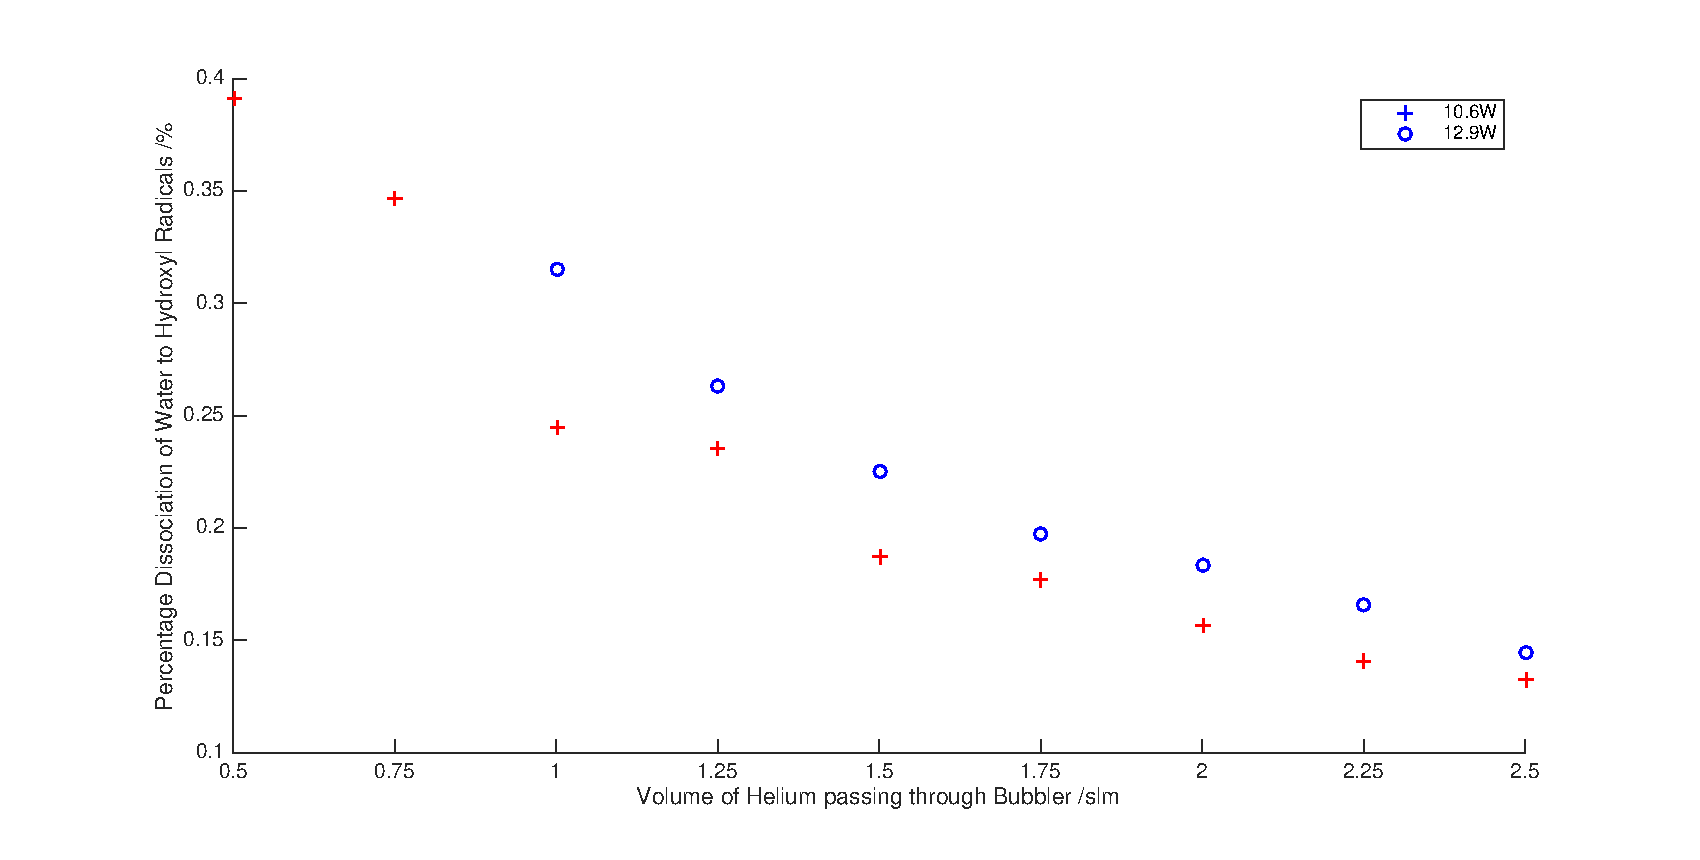
\includegraphics[width=\textwidth]{Figures/BubblerDissociation.eps}
    \caption{The percentage dissociation of water to hydroxyl radicals decreases as the water content increases. Absorption spectroscopy was carried out at a point 20mm from the gas inlet. The plasma was operated with a total of 5slm helium with water contents of 2700 - 13400 ppm. The experiment was repeated at two different powers of ??10.6 and 12.9W??.}
    \label{fig:BubblerDissociation}
\end{figure}

\begin{itemize}
    \item Percentage dissociation decreases with increasing water content, despite the density of hydroxyl radicals increasing (see figure \ref{fig:BubblerVariation}). However, the water content increases more than the density, therefore the ratio of hydroxyl radical to water still decreases.
    \item The dissociation is higher for the higher power than the lower power, as would be expected. 
    \item Dissociation may also decrease due to the increase in energy absorption by molecules. The increase in water content means that more of the energy in the plasma system can be absorbed by the molecules in rotationally and vibrationally excited states. Could add oxygen into the feed gas. In theory, oxygen addition could increase hydroxyl radical density as, when water dissociates, there is a spare hydrogen which could combine with oxygen to form hydroxyl. However, this may have the opposite effect because, once again, a molecule is being added which could contribute further to the absorption of energy from the system. The oxygen would also require energy to be atomised before it could form .OH with the spare hydrogen from water.
\end{itemize}




\section{Discussion}

Discuss lots of important things here!!!!! Woo!

\begin{itemize}
\item Increasing frequency to increase dissociation (can't increase power)
\item Change/adapt source to allow better interrogation of effluent
\item Alignment issues - improve the setup reduce error from twisting/moving of source when moving the stage vertically. Make sure everything is properly level to stop movement in x direction when moving in y direction.
\item Try to accurately identify the ends of the electrodes rather than guess
\item Test model more - change water content and see how it matches

\item Understand dose-response of plasma treatments. How long would it need to be treated and how many times? Is there a threshold for damaging host cells too much? Is it like chemotherapy needing recovery time between treatments? 
\item Selectivity. Is there a way of making these treatments selective only against bacteria, not host cells
\item Could antibiotics be aerosolised into the plasmas? Immunotherapy?!
\item Big picture - develop a plasma jet that can kill off all bacteria in a big wound in wildlife so that they can be treated once to avoid the need to capture etc

\end{itemize}

\bibliographystyle{unsrt}
\bibliography{MyPapers}

\end{document}  